\documentclass[a4paper,oneside,article]{memoir}

\usepackage{microtype}
\usepackage[UTF8]{inputenc}
\usepackage[Danish]{babel}
\usepackage[T1]{fontenc}

\setsecnumdepth{subsection}
\setcounter{tocdepth}{5}
\setcounter{secnumdepth}{5}

\usepackage{longtable}
\usepackage{lmodern}
\usepackage{array}
\usepackage{mathtools}
\usepackage{gensymb}

%Billeder skal
\usepackage{graphicx}
\usepackage[table,xcdraw]{xcolor}
\graphicspath{ {Afsnit/} }
\usepackage{float}
\usepackage{wrapfig}

% Listings og color bruges til at vise vores VHDL kode med.
\usepackage{listings}
\usepackage{color}

\usepackage{longtable}
\usepackage{tabularx}


\usepackage{natbib}

\usepackage[hidelinks=true]{hyperref}

\definecolor{dkgreen}{rgb}{0,0.6,0}
\definecolor{gray}{rgb}{0.5,0.5,0.5}
\definecolor{mauve}{rgb}{0.58,0,0.82}

\lstset{frame=tb,
  language=C++,
  aboveskip=3mm,
  belowskip=3mm,
  showstringspaces=false,
  columns=flexible,
  basicstyle={\small\ttfamily},
  numbers=none,
  numberstyle=\tiny\color{gray},
  keywordstyle=\color{blue},
  commentstyle=\color{dkgreen},
  stringstyle=\color{mauve},
  breaklines=true,
  breakatwhitespace=true,
  tabsize=3
}

%This part is just for fun! Please delete before turn-in
%=======================================================
\usepackage{transparent}
\usepackage{eso-pic}
\newcommand\BackgroundPic{%
	\put(0,0){%
		\parbox[b][\paperheight]{\paperwidth}{%
			\vfill
			\centering
			{\transparent{0.4} 
\includegraphics[width=\paperwidth,height=\paperheight]{background}}
			\vfill
		}}}
%=======================================================

\title{3. Semesterprojekt - Goofy Candy Gun\\ Dokumentation - Gruppe 3}

\author{
  Rieder, Kasper\\
  \texttt{201310514}
  \and
  Jensen, Daniel V.\\
  \texttt{201500152}
  \and
  Nielsen, Mikkel\\
  \texttt{201402530}
  \and
  Kjeldgaard, Pernille L.\\
  \texttt{PK94398}
  \and
  Konstmann, Mia\\
  \texttt{201500157}
  \and
  Kloock, Michael\\
  \texttt{201370537}
  \and
  Rasmussen, Tenna\\
  \texttt{201406382}
}

\pagestyle{headings}

\usepackage{parskip}

\begin{document}
	
	\frontmatter
	\maketitle

	\newpage
	
	\tableofcontents
	
	\newpage
	\listoffigures
	\newpage
	
	\mainmatter
	
%	\chapter{Resumé}
Denne rapport beskriver semesterprojektet for tredjesemesterstuderende, hvor en prototype for spillet Goofy Candygun 3000 er slut produktet. Ideen bag Goofy Candygun 3000 er et spilsystem hvor en eller to spillere skyder en slikkanon efter et mål for at opnå det største antal point. Brugeren interagerer med systemet gennem en touch skærm og en Wii-Nunchuck. Til projektet har IHA stillet nogle krav til hvilke elementer systemet skal indeholde. Dette inkluderer en indlejret linux platform, en sensor, en aktuator og en PSoC platform. \newline

\noindent Følgende denne rapport er en procesrapport der beskriver gruppens brug af udviklingsmodellen scrum. Derudover beskriver rapporten udviklingsforløbet af projektet samt de værktøjer der er blevet anvendt til at fremme processen. \newline

\noindent Prototypen består af et netværk af PSoC4 udviklingsboards og en Wii-Nunchuck, som kommunikerer via I2C kommunikationsprotokollen. Brugeren interagerer med systemet gennem en grafisk brugergrænseflade på Devkit 8000's touch skærm. Via Wii-Nunchuck kan brugeren kontrollere kanonens sigte, samt affyre skud. \newline

\noindent Ikke alle dele af produktet er fuldt implementeret. Implementationen af hoved use casen, som omhandler selve spillet, er påbegyndt, men ikke færdigimplementeret. Gennem prioritering med MoSCoW princippet er kommunikationen mellem linux og PSoC platformene blevet prioriteret højest og dermed er use casen omkring systemtesten blevet færdigimplementeret.

\chapter{Abstract}
This paper describes the third semester project, in which a prototype for Goofy Candygun 3000 is the final product. The vision behind Goofy Candygun 3000 is game system where one or two players aim a candycannon at a target to score the highest amount of points. The system is controlled by the user through a touch screen and a Wii-Nunchuck. For this project IHA has required that the system includes an embedded linux platform, a sensor, an actuator and a PSoC platform. \newline

\noindent Mainly, the paper describes the design and implementation of a prototype for Goofy Candygun 3000. Following this paper, a report about the usage of the agile development framework, scrum, and the group's workprocess throughout the project cycle is described. \newline 

\noindent The prototype consists of a network PSoC4's, which communicate amongst each other via the I2C communication protocol. The user interacts with the system through a graphical interface on the Devkit 8000's touch screen. Via the Wii-Nunchuck the user controls cannon's position and launches the cannon. \newline

\noindent The prototype has not been implemented fully. The implementation of the main use case, which addresses gameplay functionalities, has not been fully implemented. Using the MoSCoW method, communication amongst the linux and PSoC platforms has been prioritized highly and therefore the use case addressing the systemtest has been implemented in full.    

%Abstract er sendt til Gunvor for gennemlæsning og vurdering af længden og hvilke dele, der evt. kan udelades.
%This project aims to develop a candygun ment for use at parties and at leisure time. The finished product is to be controlled with a touchscreen for initiation of the system and a wii-nunchuck for adjusting and firing the gun. Furthermore, as demanded by predefined requirements,  an embedded linux platform is included. For this purpose the Devkit 8000 is chosen. Further predefined requirements include use of sensors and actuators and well as the use of a PSoC is required - here a PSoC4 is chosen. \\
%Through the analysis and specification of use cases the functional demands of the system are determined, then prioritized by the use of the MoSCoW-method. In the development of the project the agile development framework, Scrum, is chosen. By working incremental and iterative in the course of sprints the development has been well structured and reflected upon. The architecture of the system is described by use of the SysML. Through analysis of the communication between sub-systems protocols for I2C- and SPI has been developed. \\ 
%The end-result of this project is a prototype whose hardware include motor control of three motors and three detectors, one which makes use of a potentiometer to limit horizontal rotation of the gun, another using a photodiode for an optical detection in the firing of the gun. The last, a Wii-nunchuck reacting to user input. The hardware is closely connected to mechanic parts, who enable rotation and firing of the gun. As far as embedded software goes a big part is the implementation of the two communication systems, SPI and I2C. An eventbased graphical user interface makes up the touchscreen functionalities. And the programming of 3 PSoC4s connect the parts to complete the system. \\
%All parts meet the requirements to test the communication protocols of the system. Playing of the game with shooting the gun meets the requirements to adjust and fire the gun, but is decoupled from the touchscreen initiation of the game, though an illustrational GUI for the game has been implemented. As a results requirements for the acceptance test, with few exceptions, has been met. \newline

%	\chapter{Indledning}
Hensigten med dette projekt, er at udvikle spillet "Goofy Candygun 3000". Spillet går ud på at 1-2 spillere dyster om, at ramme et mål med slik, affyret fra en slikkanon, styret af en Wii-Nunchuck controller. For at finde inspiration til projektet, og idéer til implementering, blev der søgt efter lignende projekter på internettet. Det viste sig, at idéen med at skyde med slik, ikke er en original idé, da lignende projekter såsom "The Candy Canon" \cite{Website:CandyCanon} allerede findes. Til forskel fra The Candy Cannon og lignende projekter som affyrer projektiler uden et egentlig formål, vil der i dette projekt blive udviklet en kanon til brug i et spil. Kanonen affyres og styres af spillerne via en controller. Altså skal projektet ende med en kanon som indgår i et to personersspil, f.eks. til brug ved fester og andre sociale begivenheder.
Målet med projektet, er at bygge en funktionelt prototype, samt at dokumentere dette med en projektrapport og dens dertilhørende dokumentation. 
Det følgende afsnit beskriver, hvilke krav der stilles til projektet fra IHA's side.

\section{Krav til produktet}
Projektet tager udgangspunkt i projektoplægget for 3. Semester projektet, præsenteret af \textit{Ingeniørhøjskolen, Aarhus Universitet}. Til dette projekt er der ikke stillet krav til typen af produkt der skal udvikles, dog er der sat krav til hvad produket skal indeholde. Disse krav er som følger:


\begin{itemize}
	\item{Systemet \textit{skal} via sensorer/aktuatorer interagere med omverdenen}
	\item{Systemet \textit{skal} have en brugergrænseflade}
	\item{Systemet \textit{skal} indeholde faglige elementer fra semesterets andre fag}
	\item{Systemet \textit{skal} anvende en indlejret Linux platform og en PSoC platform}
\end{itemize}

\noindent På baggrund af disse krav er der udarbejdet et produkt, der beskrives i afsnit \ref{afsnit:systembeskrivelse}. \newline

\noindent I dette projekt bliver produktet opbygget som en prototype. Grundet dette er der i afsnit \ref{afsnit:analyse} beskrevet nogle grundlæggende hardwarekomponenter til realisering af denne prototype.


\section{Systembeskrivelse}
\label{afsnit:systembeskrivelse}
I dette projekt skal der udvikles en slik kanon, som skal bruges i et nyt spil som kommer til at hedde \textit{Goofy Candygun 3000}. Denne slik kanon skal kunne skyde med slik, eksempelvis M\&M’s eller Skittles. Kanonen der afyrer slikket, skal styres af spillerne via en Wii-Nunchuck controller.  \newline

\noindent Et typisk brugerscenarie er, at spillerne bestemmer antallet af skud for runden. Når dette er gjort, er spillet igang. Herefter går Wii-nunchucken på skift mellem spillerne for hvert skud. Dette fortsættes indtil skuddene er opbrugt. Vinderen er spilleren med flest point. Spillets statistikker vises løbende på brugergrænsefladen. Dette brugerscenarie er illustreret i det rige billede på figur \ref{fig:RigtBillede}.

\begin{figure}[H]
	\centering
	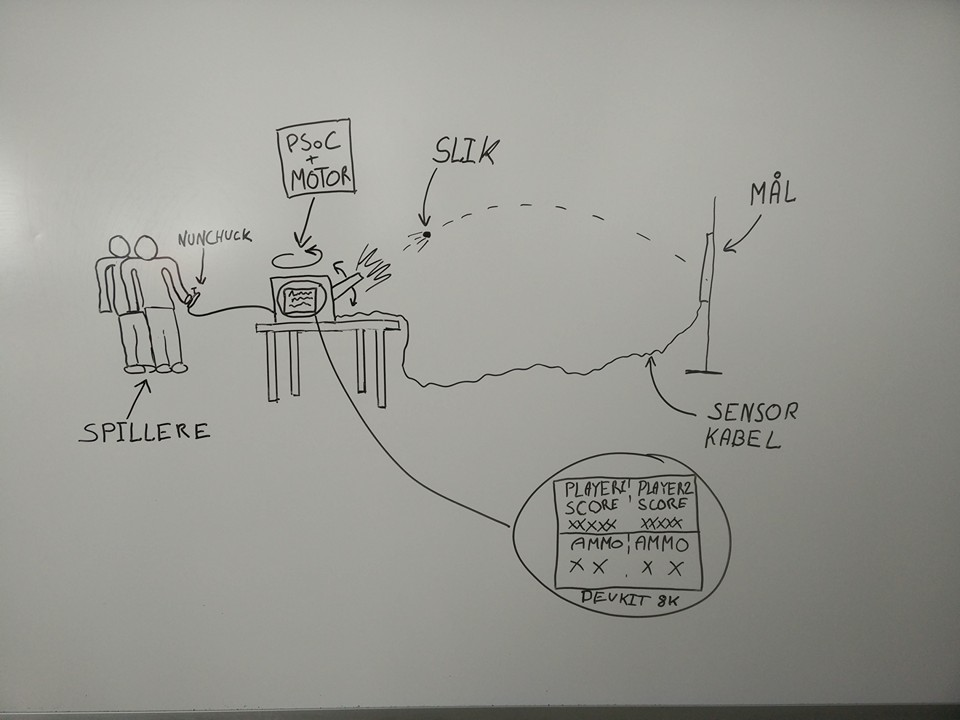
\includegraphics[width=\textwidth]{Projektformulering/images/rigtBillede}
	\caption{Rigt Billede af det endelige produkt}
	\label{fig:RigtBillede}
\end{figure}

Det endelige produkt omfatter:
\begin{itemize}
	\item{En brugergrænseflade, hvor brugeren kan initiere både system test og selve spillet. Derudover kan brugergrænsefladen vise:}
	\subitem{Point}
	\subitem{Kanonens vinkel}
	\subitem{Antal resterende skud}
	\item{Består af 3 motorer, der drejer kanonen om forskellige akser}
	\subitem{Disse skal styres med en Wii-nunchuck controller}
	\subitem{To af motorerne styre kanonen i forskellige retninger og den sidste er til at afyrer kanonen}
	\item{Et mål, der kan registrere spillernes skud}
	\item {Der skal være mulighed for at flere spille kan spille sammen, i stedet for kun 2}
\end{itemize}


%\section{Ansvarsområder}
%I løbet af projektet vil projektgruppen blive opdelt i to hovedgrupper - 'hardware' og 'software'. Softwaregruppen vil desuden stå for grænsefladeprogrammering mellem software og hardware. Disse grupper vil have til ansvar at designe og implementere hhv. hardware og software til projektet. Hardwaregruppen vil bestå af de personer, der læser til elektroingeniør (Mikkel Nielsen og Pernille Kjeldgaard). Softwaregruppen vil bestå af de personer, der læser til IKT-ingeniør (Kasper Rieder, Michael Kloock, Tenna Rasmussen, Mia Konstmann og Daniel Jensen).

%	\frontmatter
\maketitle
%=======================================================
\AddToShipoutPicture*{\BackgroundPic}
%=======================================================
\newpage

\tableofcontents
%=======================================================
\begin{figure}[h]
	
\includegraphics[width = \textwidth]{/Projektformulering/Images/goofy-study}
\end{figure}
%=======================================================
\newpage
\listoffigures
\newpage

\mainmatter


\chapter{Projektformulering}
\subsection{Indledning}
I dette projektet skal der udvikles en slikkanon til spillet Goofy Candygun 2016. Denne slikkanon skal kunne skyde med slik. Dette kunne for eksempel være M\&M’s eller Skittle’s.

Goofy Candygun 2016 er et spil til to personer. Spillet går ud på at opnå flest point ved at ramme et mål. Hver spiller får et bestemt antal skud. Efter skuddene er opbrugt er vinderen den spiller med flest point.
\begin{wrapfigure}{r}{0.2\textwidth}
	
\includegraphics[width = 0.2\textwidth]{/Projektformulering/Images/goofy}
\end{wrapfigure}

Det endelige produkt omfatter:
\begin{itemize}
	\item{En brugergrænseflade, hvor spilstatistikker fremvises til deltagerne. Dette er blandt andet:}
	\subitem{Pointvisning}
	\subitem{Kanonens vinkel}
	\subitem{Antal resterende skud}
	\item{En motor, der drejer kanonen om forskellige akser}
	\subitem{Dette styres med en Wii-nunchuck}
	\item{Et mål, der kan registrere spillernes skud}
\end{itemize}

Et typisk brugerscenarie er at spillerne bestemmer antallet af skud for runden. Når dette er gjort, er spillet igang. Herefter går Wii-nunchucken på skift mellem spillerne for hvert skud. Dette fortsættes indtil skuddene er opbrugt. Vinderen er spilleren med flest point. Spilletsstatistikker vises løbende på brugergrænsefladen. 

\begin{itemize}
	\item{rigt billede + beskrivelse}
\end{itemize}


\subsection{MoSCoW}
\begin{itemize}
	\item{Produktet must have:}
	\subitem{En motor til styring af kanonen}
	\subitem{En brugergrænseflade til visning af statistikker}
	\subitem{En Wii-nunchuck til styring af motoren}
	\subitem{En kanon med en afskydningsmekanisme der kan styres af Wii-nunchuck}
	\item{Produktet should have:}
	\subitem{Et mål til registering af point} 
	\subitem{En lokal rangliste statistik}
	\item{Produktet could have:}
	\subitem{Party mode indstilling til over to spillere}
	\subitem{Trådløs Wii-nunchuck styring}
	\subitem{Afspilning af lydeffekter}
	\item{Produktet won't have:}
	\subitem{Et batteri til brug uden strømforsyning}
	\subitem{Online rangliste statistik}	
\end{itemize}

\begin{wrapfigure}{R}{0.2\textwidth}
	
\includegraphics[width = 0.2\textwidth]{/Projektformulering/Images/goofy-write}
\end{wrapfigure}
\subsection{Opdeling af gruppen}
I løbet af projektet vil vi dele projektgruppen op i 2 hovedgrupper, nemlig 'Hardware' og 'Software'. Disse grupper vil have til ansvar at designe og implementere hhv. hardware og software til projektet. Hardware gruppen vil bestå af de folk der går på Elektro-ingeniør linjen (Mikkel Nielsen og Pernille Kjeldgaard). Softwaregruppen vil bestå af de folk der går på IKT-linjen (Kasper Rieder, Michael Kloock, Tenna Rasmussen, Mia Konstmann \& Daniel Jensen).
\begin{itemize}
	\item{Ansvarsområder}
\end{itemize}

%\begin{figure}[H]
%	
\includegraphics[width = \textwidth]{/Projektformulering/Images/goofy-cool}
%\end{figure}

%	\include{Afsnit/Projektafgraensning/Projektafgraensning}
%	\include{Afsnit/Systembeskrivelse/Systembeskrivelse}
	\documentclass{article}

% -- PREAMBLE START --
\usepackage[utf8]{inputenc}
\usepackage[T1]{fontenc}
\usepackage{lmodern} % load a font with all the characters

\usepackage{parskip}

\usepackage[danish]{isodate}

\usepackage{array}

\begin{document}
	\title{Kravspecifikation}
	\maketitle
	
	\section{Fully dressed use case}
	\begin{tabular}{|>{\hspace{0pt}}p{3cm}  |>{\hspace{0pt}}p{9cm}|}
		\hline
		\textbf{Navn} & Spil Goofy Candygun 3000\\ \hline
		\textbf{Mål} & At spille spillet\\ \hline
		\textbf{Initiering} & Bruger\\ \hline
		\textbf{Aktører} & Bruger\\ \hline
		\textbf{Antal samtidige forekomster} & Ingen \\ \hline
		\textbf{Prækondition} & Spillet og kanonen er operationelt \\ \hline
		\textbf{Postkondition} &  Brugeren har færdiggjort spillet \\ \hline
		\textbf{Hovedscenarie} & \begin{enumerate}
			\item Bruger vælger spiltype på brugergrænsefladen
			\subitem [Extension 1: Brugeren vælger 2 player mode] 
			\item Brugeren vælger antal skud til runden
			\item Brugeren fylder magasin med slik tilsvarende antal skud
			\item Brugeren indstiller kanon med analog stick på Wii-nunchuck
			\item Bruger udløser kanonen med Wii-nunchucks trigger
			\item Brugergrænsefladen opdateres med spillets statistikker
			\item Punkt 4 til 6 gentages indtil skuddene er opbrugt 
			\subitem[Extension 2: Bruger afslutter det igangværende spil]
			\item Brugergrænseflade viser afslutningsinfo for runden
			\item Brugeren afslutter runden
			\item Brugergrænsefladen vender tilbage til starttilstanden
		\end{enumerate}\\ \hline
		\textbf{Udvidelser/ undtagelser} & \textbf{[Extension 1: Brugeren vælger 2 player mode]} \newline \begin{enumerate} 
			\item Punkt 4 til 6 i hovedscenariet gennemføres
			\item Brugeren overdrager Wii-nunchuck til den anden bruger
			\item Punkt 1 til 2 gentages indtil skuddene er opbrugt
			\item Use casen genoptages fra punkt 8
			\end{enumerate}
			\textbf{[Extension 2: Bruger afslutter det igangværende spil]} \newline \begin{enumerate}
			\item Brugergrænsefladen vender tilbage til starttilstanden
			\item Use casen afsluttes
			\end{enumerate}\\ \hline
	\end{tabular}
\end{document}
	\chapter{Accepttestspecifikation}

\section{Use case 1 - Hovedscenarie}
\begin{tabular}{|>{\hspace{0pt}}p{0.6cm} |  >{\hspace{0pt}}p{3.5cm} | >{\hspace{0pt}}p{2.5cm} | p{2.5cm} | p{2cm} |}
	\hline
	Step & Handling & Forventet observation/resultat& Faktisk observation/resultat & Vurdering (OK/FAIL)\\ \hline
	1 & Vælg one-player mode. & Brugergrænsefladen viser spilside for one-player mode og anmoder om valg af antal skud. & & \\ \hline
	
	2 & Vælg ti skud. & Brugergrænseflade anmoder om, at der fyldes ti stykker slik i magasin. & & \\ \hline
	
	3 & Fyld ti stykker slik i magasinet og tryk på knap for at starte spil. & Brugergrænseflade går til spilside og anmoder om, at kanon indstilles. & & \\ \hline
	
	4 & Indstil kanon til affyring med Wii-nunchuck. & Kanon indstiller sig svarende til Wii-nunchucks placering. & & \\ \hline
	
	5 & Udløs kanon med trigger på wii-nunchuck. & Kanon udløses. & & \\ \hline
	
	6 & Gentag punkt 4 og 5 ti gange.  & Punkt 4 og 5 gentages.  & & \\ \hline
	
	7 & Kig på brugergrænsefladen. & Brugergrænsefladen viser info om spillet. & & \\ \hline
	
	8 & Tryk på knap for at vende tilbage til starttilstand. & Brugergrænseflade vender tilbage til startside. & & \\ \hline
\end{tabular}

\subsection{Use case 1 - Extension 1}
\begin{tabular}{|>{\hspace{0pt}}p{0.6cm} |  >{\hspace{0pt}}p{3.5cm} | >{\hspace{0pt}}p{2.5cm} | p{2.5cm} | p{2cm} |}
	\hline
	Step & Handling & Forventet observation/resultat& Faktisk observation/resultat & Vurdering (OK/FAIL)\\ \hline
	
	1 & Vælg two-player mode. & Brugergrænsefladen viser spilside for two-player mode og anmoder om valg af antal skud. & & \\ \hline
	
	2 & Vælg ti skud på brugergrænseflade. & Brugergrænseflade anmoder om, at der fyldes ti stykker slik i magasin. & & \\ \hline
	
	3 & Fyld ti stykker slik i magasinet og tryk på knap for at starte spil. & Brugergrænseflade går til spilside og anmoder om, at kanon indstilles. & & \\ \hline
	
	4 & Indstil kanon til affyring med Wii-nunchuck. & Kanon indstiller sig svarende til Wii-nunchucks placering. & & \\ \hline
	
	5 & Udløs kanon med trigger på wii-nunchuck. & Kanon udløses. & & \\ \hline
	
	6 & Giv Wii-nunchuck til den anden spiller. & Den anden spiller modtager Wii-nunchuck.  & & \\ \hline
	
	7 & Gentag punkt 4 til 6 indtil skud er opbrugt. & Punkt 4 til 6 gentages. & & \\ \hline
	
	8 & Kig på brugergrænseflade. & Brugergrænseflade viser info om spil. & & \\ \hline
	
	9 & Tryk på knap for at vende tilbage til starttilstand. & Brugergrænseflade vender tilbage til startside. & & \\ \hline
\end{tabular}

\subsection{Use case 1 - Extension 2}
\begin{tabular}{|>{\hspace{0pt}}p{0.6cm} |  >{\hspace{0pt}}p{3.5cm} | >{\hspace{0pt}}p{2.5cm} | p{2.5cm} | p{2cm} |}
	\hline
	Step & Handling & Forventet observation/resultat& Faktisk observation/resultat & Vurdering (OK/FAIL)\\ \hline
	
	1 & Vælg one-player mode. & Brugergrænsefladen viser spilside for one-player mode og anmoder om valg af antal skud. & & \\ \hline
	
	2 & Vælg ti skud på brugergrænseflade. & Brugergrænseflade anmoder om, at der fyldes ti stykker slik i magasin. & & \\ \hline
	
	3 & Fyld ti stykker slik i magasinet og tryk på knap for at starte spil. & Brugergrænseflade går til spilside og anmoder om, at kanon indstilles. & & \\ \hline
	
	4 & Tryk på knap for afslutning af spil. & Brugergrænseflade vender tilbage til startside. & & \\ \hline
\end{tabular}

\section{Use case 2 - Hovedscenarie}
\begin{table}[H]
	\centering
	\begin{tabular}{|l|l|l|l|l|}
		\hline
		Step & Handling                                                                        & \begin{tabular}[c]{@{}l@{}}Forventet \\ observation/resultat\end{tabular}                                                                                                          & \begin{tabular}[c]{@{}l@{}}Faktisk \\ observation/resultat\end{tabular} & \begin{tabular}[c]{@{}l@{}}Vurdering \\ (OK/FAIL)\end{tabular} \\ \hline
		1.   & \begin{tabular}[c]{@{}l@{}}Tryk på \\ "Systemtest" \\ på GUI\end{tabular}                 & \begin{tabular}[c]{@{}l@{}}Systemtest brugergrænsefladen\\ vises på Devkittet.\end{tabular}                                                                                        &                                                                         &                                                                \\ \hline
		2.   & \begin{tabular}[c]{@{}l@{}}Tryk på \\ "Start Test \\ på GUI"\end{tabular}                 & \begin{tabular}[c]{@{}l@{}}Brugergrænsefladen udskriver\\ at SPI og I2C testen er\\ godkendt. Brugergrænsefladen\\ anmoder brugereren \\ om tryk på Z på Wii-nunchuck\end{tabular} &                                                                         &                                                                \\ \hline
		3.   & \begin{tabular}[c]{@{}l@{}}Tryk 'Z' knappen\\ på \\ Wii-nunchucken\end{tabular} & \begin{tabular}[c]{@{}l@{}}Brugergrænsefladen udskriver\\ at Wii-testen er godkendt\end{tabular}                                                                                   &                                                                         &                                                                \\ \hline
	\end{tabular}
\end{table}

\subsection{Use case 2 - Exception 1}
\begin{table}[H]
	\centering
	\begin{tabular}{|l|l|l|l|l|}
		\hline
		Step & Handling                                                                 & \begin{tabular}[c]{@{}l@{}}Forventet \\ observation/resultat\end{tabular}                                   & \begin{tabular}[c]{@{}l@{}}Faktisk \\ observation/resultat\end{tabular} & \begin{tabular}[c]{@{}l@{}}Vurdering \\ (OK/FAIL)\end{tabular} \\ \hline
		1.   & \begin{tabular}[c]{@{}l@{}}Fjern SPI-kablet\\ fra Devkittet\end{tabular} &                                                                                                             &                                                                         &                                                                \\ \hline
		2.   & \begin{tabular}[c]{@{}l@{}}Tryk på \\ "Systemtest" \\ på GUI \end{tabular}          & \begin{tabular}[c]{@{}l@{}}Systemtest bruger-\\ grænsefladen\\ vises på Devkittet.\end{tabular}             &                                                                         &                                                                \\ \hline
		3.   & \begin{tabular}[c]{@{}l@{}}Tryk på \\ "Start Test" \\ på GUI\end{tabular}          & \begin{tabular}[c]{@{}l@{}}Brugergrænsefladen \\ udskriver at\\ SPI forbindelsen\\ mislykkedes\end{tabular} &                                                                         &                                                                \\ \hline
	\end{tabular}
\end{table}


\subsection{Use case 2 - Exception 2}
\begin{table}[H]
	\centering
	\begin{tabular}{|l|l|l|l|l|}
		\hline
		Step & Handling                                                                 & \begin{tabular}[c]{@{}l@{}}Forventet \\ observation/resultat\end{tabular}                                   & \begin{tabular}[c]{@{}l@{}}Faktisk \\ observation/resultat\end{tabular} & \begin{tabular}[c]{@{}l@{}}Vurdering \\ (OK/FAIL)\end{tabular} \\ \hline
		1.   & \begin{tabular}[c]{@{}l@{}}Fjern I2C-kabel\\ fra PSoC0\end{tabular}      &                                                                                                             &                                                                         &                                                                \\ \hline
		2.   & \begin{tabular}[c]{@{}l@{}}Tryk på \\ "Systemtest"\\ på GUI\end{tabular} & \begin{tabular}[c]{@{}l@{}}Systemtest bruger-\\ grænsefladen\\ vises på Devkittet.\end{tabular}             &                                                                         &                                                                \\ \hline
		3.   & \begin{tabular}[c]{@{}l@{}}Tryk på \\ "Start Test"\\ på GUI\end{tabular} & \begin{tabular}[c]{@{}l@{}}Brugergrænsefladen \\ udskriver at\\ SPI forbindelsen\\ lykkedes og \\ I2C forbindelsen \\ mislykkedes\end{tabular} &                                                                         &                                                                \\ \hline
	\end{tabular}
\end{table}

\subsection{Use case 2 - Exception 3}
\begin{table}[H]
	\centering
	\begin{tabular}{|l|l|l|l|l|}
		\hline
		Step & Handling                                                                     & \begin{tabular}[c]{@{}l@{}}Forventet \\ observation/resultat\end{tabular}                                        & \begin{tabular}[c]{@{}l@{}}Faktisk \\ observation/resultat\end{tabular} & \begin{tabular}[c]{@{}l@{}}Vurdering \\ (OK/FAIL)\end{tabular} \\ \hline
		1.   & \begin{tabular}[c]{@{}l@{}}Afkobl Nun-\\ chucken\\ fra systemet\end{tabular} &                                                                                                                  &                                                                         &                                                                \\ \hline
		2.   & \begin{tabular}[c]{@{}l@{}}Tryk på \\ "Systemtest"\\ på GUI\end{tabular}     & \begin{tabular}[c]{@{}l@{}}Systemtest bruger-\\ grænsefladen\\ vises på Devkittet.\end{tabular}                  &                                                                         &                                                                \\ \hline
		3.   & \begin{tabular}[c]{@{}l@{}}Tryk på \\ "Start Test"\\ på GUI\end{tabular}     & \begin{tabular}[c]{@{}l@{}}Brugergrænsefladen \\ udskriver at\\ SPI og I2C forbindelsen\\ lykkedes\end{tabular}  &                                                                         &                                                                \\ \hline
		4.   & Afvent timeout                                                               & \begin{tabular}[c]{@{}l@{}}Brugergrænsefladen \\ udskriver at\\ Nunchuck forbindelsen\\ mislykkedes\end{tabular} &                                                                         &                                                                \\ \hline
	\end{tabular}
\end{table}


\section{Ikke-funktionelle krav}
\begin{tabular}{|>{\hspace{0pt}}p{0.6cm} |  >{\hspace{0pt}}p{3.5cm} | >{\hspace{0pt}}p{2.5cm} | p{2.5cm} | p{2cm} |}
	\hline
	Krav & Test & Forventet observation/resultat& Faktisk observation/resultat & Vurdering (OK/FAIL)\\ \hline
	
	1 & Bruger drejer kanonen så lang til venstre og højre som muligt. & Det observeres at kanonen ikke har roteret 360 \degree  & & \\ \hline
	
	2 & Et projektil på 1.25 cm i diameter \(\pm\) 5mm affyres fra kanonen. & Projektilet bliver affyret & & \\ \hline
	
	3 & Et projektil affyres, og distancen mellem kanonen og stedet hvor projektilet lander måles. & Distancen er blevet målt til at være større end 1 meter. & & \\ \hline
	
	4 & Mål kanonens dimensioner med en lineal. & Dimensionerne overstiger ikke 50cm x 50cm x 50cm. & & \\ \hline
	
	5 & Tryk på 'Z' knappen på Wii Nunchuck, og mål med et stopur hvor lang tid der går fra tryk, til kanonen bliver affyret. &Den målte tid er mindre end 10 sekunder. & & \\ \hline
	
	6 & Kanonen affyres 3 gange, og et stopur startes ved første skud, og stoppes ved det tredje skud. &Den målte tid er mindre end 60 sekunder. & & \\ \hline
	
\end{tabular}
%	\include{Afsnit/Projektbeskrivelse/Projektbeskrivelse}
	\chapter{Systemarkitektur}
Systemarkitekturen har til formål at beskrive både hardware- og softwarekomponenter til sådan en grad at sammensætningen af hele system kan forstås. I dette afsnit beskrives arkitektur for både hardware og software.

I hardwarearkitekturen beskrives systemet ved at nedbryde det i blokke. I BDD'et er blokkenes porte og associationer til andre blokke angivet. Disse porte anvendes senere i afsnittet, hvor de benyttes i IBD'et.

I softwarearkitekturen udarbejdes der applikationsmodeller bestående af sekvensdiagrammer og klassediagrammer for hver use case, opdelt for hver CPU i systemet. Applikationsmodellerne har til formål at danne et overblik af de krav der stilles til softwaren for produktets uses cases. På denne måde kan de bruges som inspirerende grundlæg for software design og implementering. Applikationsmodellerne giver en overfladisk beskrivelse af CPU'ernes interaktioner.

\section{Domæne model}
På figur \ref{fig:DomainModel} ses domæne modellen for systemet. Denne er lavet for at danne et overblik over systemet, og hvordan de forskellige dele overfladisk interagerer med hinanden. 

\begin{figure}[H]
	\centering
	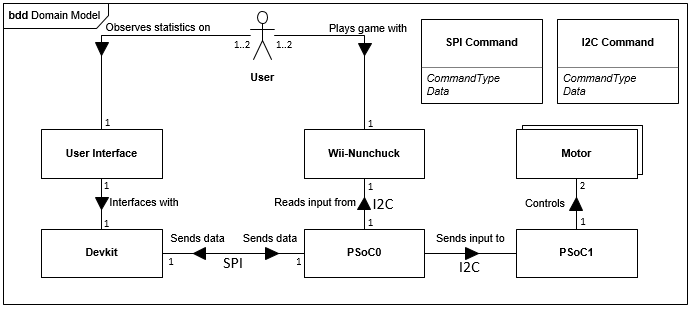
\includegraphics[width=\textwidth]{Systemarkitektur/images/DomainModel}
	\caption{Domæne model for Candygun 3000}
	\label{fig:DomainModel}
\end{figure}

I domæne modellen ses, at brugeren interagerer med både Wii-nunchucken og med brugergrænsefladen. Brugergrænsefladen er en grænseflade til softwaren devkittet. Devkittet kommunikerer med PSoC0, som læser den analoge data der kommer fra Wii-nunchucken. Denne data bliver derefter afkodet og videresendt til PSoC1, som styrer motorene ud fra dataene. PSoC1 sender også et interrupt til PSoC2, når 'Z' knappen på nunchucken bliver trykket. Når PSoC2 modtager interruptet, starter motoren for affyringsmekanismen i projectile launcher.


I "I2C Command" ses en grov estimering af interfacet mellem de forskellige I2C enheder i systemet. Commandtype bruges til at identificere hvilken data der bliver sendt. Data er en mængde tal-værdier der bliver tolket ud fra hvilken commandtype der er blevet sendt.

I "SPI Command" ses en estimering af interfacet mellem SPI enhederne i systemet. "Commandtype" bruges til at identificere hvilken opgave systemet skal udføre (f.eks. 'I2C-test'). Data kan indeholde tal-værdier, som repræsenterer nunchuck værdier (buttonpress osv.). 
En mere detaljeret gennemgang af disse kommunikations protokoller kan findes i afsnit \ref{afsnit:kommunikationsprotokoller} - Kommunikationsprotokoller.

% ---------------BDD--------------------------------------------------
\section{BDD for Candygun 3000}
På figur \ref{fig:BDD} ses et \textit{Block Definition Diagram (BDD)} 
Figur \ref{fig:BDD} skal give et overblik over hvordan  relationerne mellem de forskellige hardwareblokke er. Så man får et overordnet billede af hvordan strukturen er for ” Candygun 3000”. For at læse hvad hver blok skal bruges til, henvises der til tabel \ref{blokbeskrivelse} (blokbeskrivelse). Der på BDD'et figur \ref{fig:BDD} med nødvændige indgange og udgange for de fysiske signaler. Yderligere ses det at flow specifikationer er defineret for de ikke-atomare forbindelser \textit{I2C} samt \textit{SPI}, da disse er busser bestående af flere forbindelser. Der henvises til \textbf{IBD AFSNIT} for en detaljeret model af de fysiske forbindelser mellem hardwareblokkende.



\begin{figure}[H]
	\centering
	%trim = {1.8cm 14.6cm 1.8cm 1cm}, clip = true, %
	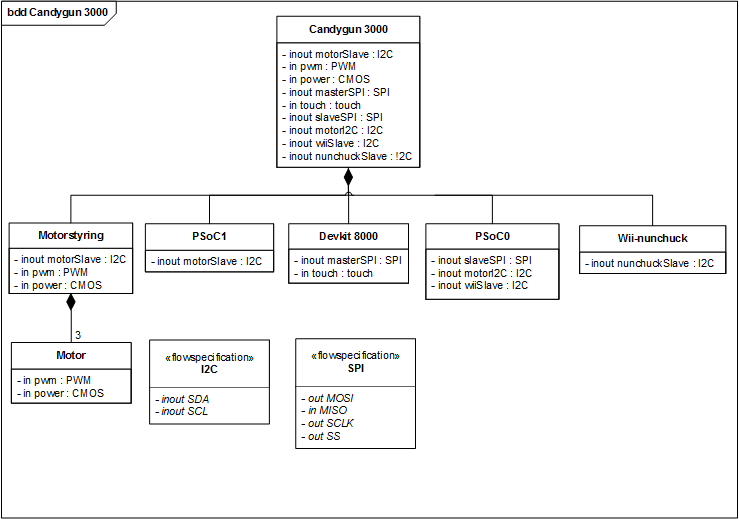
\includegraphics[width= \textwidth]{Systemarkitektur/images/BDD_overordnet.png}
	\caption{BDD for Candygun 3000}
	\label{fig:BDD}
\end{figure}


\subsection{Blokbeskrivelse}
\begin{table}[H]
	\centering
	\begin{tabular}{|l|l|}
		\hline
		\textbf{Bloknavn}       & \textbf{Beskrivelse}                                                                                                                                                                                                                           \\ \hline
		Devkit 8000             & \begin{tabular}[c]{@{}l@{}}
			DevKit 8000 er en embedded Linux platform med touch-skærm, \\ der bruges tilbrugergrænsefladen for produktet. Brugeren inter- \\ agerer med systemet og ser status for spillet via Devkit 8000.                                                      \end{tabular} \\ \hline
		Wii-Nunchuck            & \begin{tabular}[c]{@{}l@{}}Wii-Nunchuck er controlleren som brugeren styrer kanonens \\ retning med. \end{tabular} \\ \hline
		PSoC0                   & \begin{tabular}[c]{@{}l@{}}PSoC0 er PSoC hardware der indeholder software til I2C og \\ SPI kommunikationen og afkodning af Wii-Nunchuck data. \\ PSoC0 fungerer som I2C masterog SPI slave. Denne PSoC er \\ bindeleddet mellem brugergrænsefladen og restenaf systemets \\ hardware. \end{tabular} \\ \hline
		MotorControl                   & \begin{tabular}[c]{@{}l@{}}MotorControl blokken er Candy Gun 3000’s motorerer, der anvendes \\ til at bevæge kanonen. Denne blok består af H-bro blokken og \\ rotationsbegrænsnings blokken. \end{tabular} \\ \hline
		Motor &
		\begin{tabular}[c]{@{}l@{}}Motor er motorene der bruge til at bevæge platform og kanon. \end{tabular} \\ \hline
		H-bro &
		\begin{tabular}[c]{@{}l@{}}H-bro bruges til at styre mototrens rotationsretning \end{tabular} \\ \hline
		Rotationsbegrænsning &
		\begin{tabular}[c]{@{}l@{}}Rotationsbegrænsning er til at begrænse platformens rotation så \\ denne ikke kan dreje 360 grader. Den blok består af et potentiometer \\ og en ADC'en, som sidder internt på PSoC0  \end{tabular} \\ \hline
		PSoC1                   & \begin{tabular}[c]{@{}l@{}}PSoC1 er PSoC hardware der indeholder software til I2C \\ kommunikation og styring af Candy Gun 3000’s motorer. \\ PSoC1 fungerer som I2C slave. \end{tabular} \\ \hline
		SPI (FlowSpecification) &  \begin{tabular}[c]{@{}l@{}}SPI (FlowSpecification) beskriver signalerne der indgår i SPI \\ kommunikation. \end{tabular} \\ \hline
		I2C (FlowSpecification) &  \begin{tabular}[c]{@{}l@{}}I2C (FlowSpecification) beskriver signalerne der indgår i I2C \\ kommunikation. \end{tabular} \\ \hline	
		PSoC2  &  \begin{tabular}[c]{@{}l@{}}PSoC2 denne blok står for at sende et signal til\\ affyringsmekanismen om at den skal skyde og så skal den\\ også holde styre på at der kun bliver skydt en gang. \end{tabular} \\ \hline
		Projectile Launcher  &  \begin{tabular}[c]{@{}l@{}}Projectile Launcher denne blok er vores affyringsmekanismen \end{tabular} \\ \hline
	\end{tabular}
	\label{blokbeskrivelse}
	\caption{Blokbeskrivelse}
\end{table} ---------------IBD--------------------------------------------------
\section{IBD for Candygun 3000}
På baggrund af BDD'et er der lavet et \textit{Internal Block Diagram (IBD)}. I IBD'et på figur \ref{fig:IBD} ses forbindelserne og portene mellem systemets blokke. Diagrammet viser grænsefladerne mellem blokkene og flowet i mellem disse. 

\begin{figure}[H]
	\centering
	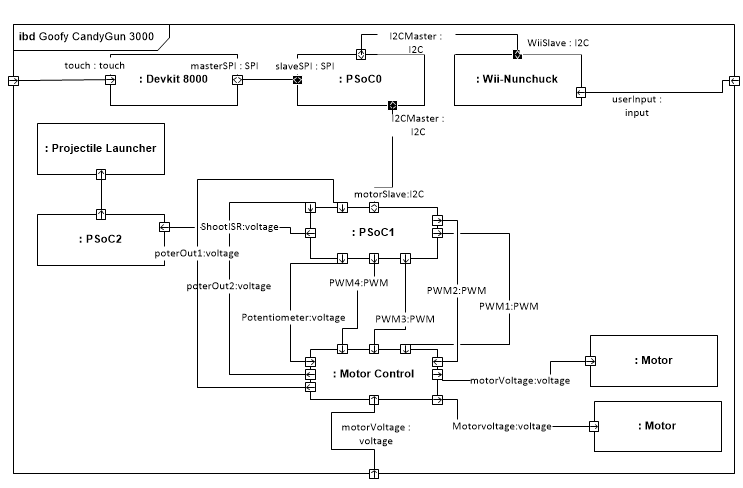
\includegraphics[width=\textwidth]{Systemarkitektur/images/jgjgj}
	\caption{IBD for Candygun 3000}
	\label{fig:IBD}
\end{figure}

\begin{figure}[H]
	\centering
	%trim = {1.8cm 14.6cm 1.8cm 1cm}, clip = true, %
	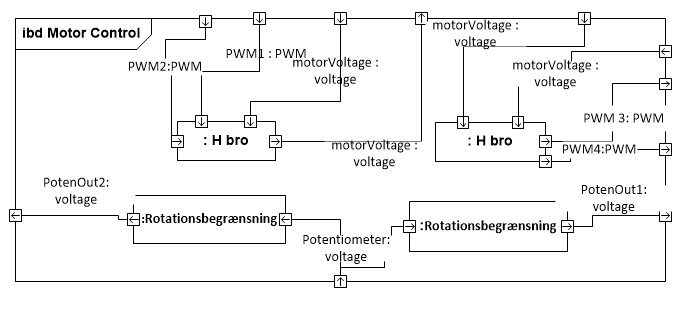
\includegraphics[width= \textwidth]{Systemarkitektur/images/IBDmotorcontrol2}
	\caption{IBD for motor control}
	\label{fig:IBDm}
\end{figure}
I IBD'et på figur \ref{fig:IBDm} ses forbindelserne og portene mellem blokkene i motorControl blokken. Diagrammet viser grænsefladerne mellem disse blokke og flowet i mellem disse.

\subsection{Signalbeskrivelse}

I signalbeskrivelsen gælder det, at når et signal beskrives som 'højt' opereres der i et spændingsområde på 3.5V til 5V. På samme måde er signaler beskrevet som 'lav' defineret som spændinger indenfor et område fra 0V til 1,5V. Disse spændingsniveauer er defineret  ud fra standarden for CMOS kredse \cite{cmosStandard}.
\begin{longtable}{|>{\hspace{0pt}}p{3cm} | >{\hspace{0pt}}p{3cm} | p{2cm} | p{3cm} |}
	\hline                                                                                                                                                         
	\textbf{Blok-navn} & \textbf{Funktionsbeskrivelse} & \textbf{Signaler} & \textbf{Signalbeskrivelse} \\ \hline
	Devkit 8000 & Fungerer som grænseflade mellem bruger og systemet samt SPI master. & masterSPI & Type: SPI \newline Spændingsniveau: 0-5V \newline Hastighed: 1Mbps \newline Beskrivelse: SPI bussen hvori der sendes og modtages data.\\ \cline{3-4}
	& & touch & Type: touch \newline Beskrivelse: Brugertryk på Devkit 8000 touchdisplay. \\ \hline
	PSoC0 & Fungerer som I2C master for PSoC1 og Wii-Nunchuck samt SPI slave til Devkit 8000. & slaveSPI & Type: SPI \newline Spændingsniveau: 0-5V \newline Hastighed: 1Mbps \newline Beskrivelse: SPI bussen hvori der sendes og modtages data.\\ \cline{3-4}
	& & wiiMaster & Type: I2C \newline Spændingsniveau: 0-5V\newline Hastighed: 100Kpbs \newline Beskrivelse: I2C bussen hvor der modtages data fra Nunchuck.\\ \cline{3-4}
	& & motorMaster & Type: I2C \newline Spændingsniveau: 0-5V \newline Hastighed: 100kbit/sekund \newline Beskrivelse: I2C bussen hvor der sendes afkodet Nunchuck data til PSoC1.\\ \hline
	PSoC1 & Modtager nunchuckinput fra PSoC0 og omsætter dataene til PWM signaler. & motorSlave & Type: I2C \newline Spændingsniveau: 0-5V \newline Hastighed: 100kbit/sekund \newline Beskrivelse: Indeholder formatteret Wii-Nunchuck data som omsættes til PWM-signal. \\ \cline{3-4} 
	&& ShootISR & Type: voltage \newline Spændingsniveau: 0-5V \newline Beskrivelse:  giv et højt signal når den skal skyde.\\ \cline{3-4}   
	& & PWM & Type: PWM \newline Frekvens: 22kHz \newline PWM \%: 0-100\% \newline Spændingsniveau: 0-5V \newline Beskrivelse: PWM signal til styring af motorens hastighed. \\ \cline{3-4}
	& & PotenOut1 & Type: voltage \newline Spændingsniveau: en spænding 0V-5V alt efter hvad potentiometer står på \newline Beskrivelse: den spænding viser hvor motoren står henne\\ \cline{3-4}
	& & PotenOut2 & Type: voltage \newline Spændingsniveau: en spænding 0V-5V alt efter hvad potentiometer står på \newline Beskrivelse: den spænding viser hvor motoren står henne\\ \cline{3-4}
	& & PWM1 & Type: PWM \newline Frekvens: 3MHz \newline PWM\%: 0-100\% \newline Spædingsniveau: 0-5V \newline Beskrivelse: PWM signal til styring af motorens hastighed. \\ \cline{3-4}
	&& PWM2 & Type: PWM \newline Frekvens: 3MHz \newline PWM\%: 0-100\% \newline Spædingsniveau: 0-5V \newline Beskrivelse: PWM signal til styring af motorens hastighed. \\ \cline{3-4}
	
	
	&& PWM3 & Type: PWM \newline Frekvens: 3MHz \newline PWM\%: 0-100\% \newline Spædingsniveau: 0-5V \newline Beskrivelse: PWM signal til styring af motorens hastighed. \\ \cline{3-4}
	&& PWM4 & Type: PWM \newline Frekvens: 3MHz \newline PWM\%: 0-100\% \newline Spædingsniveau: 0-5V \newline Beskrivelse: PWM signal til styring af motorens hastighed. \\ \cline{3-4}
	& & motorVoltage & Type: voltage \newline Spændingsniveau: 9V \newline Beskrivelse: Strømforsyning til motoren\\ \cline{3-4}
	& & potentiometer & Type: voltage \newline Spændingsniveau: 5V \newline Beskrivelse: giver Rotationsbegrænsing 5V \\ \hline
	MotorControl & Den enhed der skal bevæge kanonen & PWM1 & Type: PWM \newline Frekvens: 3MHz \newline PWM\%: 0-100\% \newline Spædingsniveau: 0-5V \newline Beskrivelse: PWM signal til styring af motorens hastighed. \\ \cline{3-4}
	&& PWM2 & Type: PWM \newline Frekvens: 3MHz \newline PWM\%: 0-100\% \newline Spædingsniveau: 0-5V \newline Beskrivelse: PWM signal til styring af motorens hastighed. \\ \cline{3-4}
	
	
	&& PWM3 & Type: PWM \newline Frekvens: 3MHz \newline PWM\%: 0-100\% \newline Spædingsniveau: 0-5V \newline Beskrivelse: PWM signal til styring af motorens hastighed. \\ \cline{3-4}
	&& PWM4 & Type: PWM \newline Frekvens: 3MHz \newline PWM\%: 0-100\% \newline Spædingsniveau: 0-5V \newline Beskrivelse: PWM signal til styring af motorens hastighed. \\ \cline{3-4}
	& & motorVoltage & Type: voltage \newline Spændingsniveau: 9V \newline Beskrivelse: Strømforsyning til motoren\\ \cline{3-4}
	& & potentiometer & Type: voltage \newline Spændingsniveau: 5V \newline Beskrivelse: giver Rotationsbegrænsing 5V 
	\\ \cline{3-4}
	& & PotenOut1 & Type: voltage \newline Spændingsniveau: en spænding 0V-5V alt efter hvad potentiometer står på \newline Beskrivelse: den spænding viser hvor motoren står henne\\ \cline{3-4}
	& & PotenOut2 & Type: voltage \newline Spændingsniveau: en spænding 0V-5V alt efter hvad potentiometer står på \newline Beskrivelse: den spænding viser hvor motoren står henne
	\\ \hline
	Motor & Denne blok beskriver hvad motoren får. & motorvoltage & Type: voltage \newline Spændingsniveau: 0-5V  \newline Beskrivelse: giver spændning til motoren.(denne beskevelse glæder også for den anden motor) \\ \hline
	Wii-nunchuck & Den fysiske controller som brugeren styrer kanonen med. & wiiSlave & Type: I2C \newline Spændingsniveau: 0-5V \newline Hastighed: 100kbit/sekund \newline Beskrivelse: Kommunikationslinje mellem PSoC1 og Wii-Nunchuck. \\ \cline{3-4}
	& & userInput & Type: input \newline Beskrivelse: Brugerinput fra Wii-Nunchuck. \\ \hline
	SPI & Denne blok beskriver den ikke-atomiske SPI forbindelse. & MOSI & Type: CMOS \newline Spændingsniveau: 0-5V \newline Beskrivelse: Binært data der sendes fra master til slave. \\ \cline{3-4}
	& & MISO & Type: CMOS \newline Spændingsniveau: 0-5V \newline Beskrivelse: Binært data der sendes fra slave til master. \\ \cline{3-4}
	& & SCLK & Type: CMOS \newline Spændingsniveau: 0-5V \newline Hastighed: 1Mbps\newline Beskrivelse: Clock signalet fra master til slave, som bruges til at synkronisere den serielle kommunikation. \\ \cline{3-4}
	& & SS & Type: CMOS \newline Spændingsniveau: 0-5V \newline  Beskrivelse: Slave-Select, som bruges til at bestemme hvilken slave der skal kommunikeres med. \\ \hline
	I2C & Denne blok beskriver den ikke-atomiske I2C forbindelse. & SDA & Type: CMOS \newline Spændingsniveau: 0-5V \newline \newline Beskrivelse: Databussen mellem I2C masteren og I2C slaver. \\ \cline{3-4}
	& & SCL & Type: CMOS \newline Spændingsniveau: 0-5V \newline Hastighed: 100kbps \newline Beskrivelse: Clock signalet fra master til lyttende I2C slaver, som bruges til at synkronisere den serielle kommunikation. \\ \hline
	PSoC2& Denne blok bindeledet mellem afyrningsmeknismen og PSoC1. & ShootISR & Type: voltage \newline Spændingsniveau: 0-5V \newline Beskrivelse:  giv et højt signal når den skal skyde.  \\ \hline
	Projectile Launcher & Denne blok er vores afyrningsmeknismen. & PWM5 & Type: PWM \newline Spændingsniveau: 0-5V \newline Beskrivelse: giver signal til mosfet til at åbne så motoren køre en omgang. \\ \hline
	\caption{Tabel med signalbeskrivelse}
\end{longtable}


\section{Software Allokeringsdiagram}
På figur \ref{fig:softwareAllocation} ses et software allokations diagram. Dette diagram danner et overblik over hvilke CPU'er der findes i systemet, og hvilken software der skal allokeres på disse. Følgende applikationsmodeller tager udgangspunkt i softwaren der allokeres i figuren.

\begin{figure}[H]
	\centering
	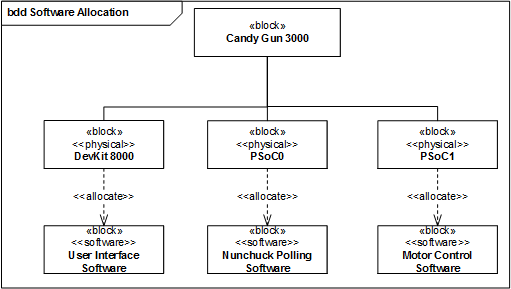
\includegraphics[width=\textwidth]{Systemarkitektur/images/SoftwareAllocation.png}
	\caption{Software allokations diagram}
	\label{fig:softwareAllocation}
\end{figure}

På tabel \ref{tabel:softwareAllocationDescription} er hvert allokeret software komponent beskrevet.

\begin{table}[H]
	\centering
	\begin{tabular}{|ll|}
		\hline
		User Interface Software   & \begin{tabular}[c]{@{}l@{}}Dette allokerede software er brugergrænsefladen\\ som brugeren interagerer med på DevKit8000 touch-skærmen.\end{tabular}                                                  \\
		\rowcolor[HTML]{CBCEFB} 
		Nunchuck Polling Software & \begin{tabular}[c]{@{}l@{}}Dette allokerede software har til ansvar at polle\\ Nunchuck tilstanden og videresende det til\\ PSoC1.\end{tabular}                                                      \\
		Motor Control Software    & \cellcolor[HTML]{FFFFFF}\begin{tabular}[c]{@{}l@{}}Dette allokerede software har til ansvar at\\ bruge den pollede Nunchuck data fra PSoC0\\ til motorstyring samt affyringsmekanismen.\end{tabular} 
		\\ 
		\rowcolor[HTML]{CBCEFB} 
		Projectile Launcher Software & \begin{tabular}[c]{@{}l@{}}Dette allokerede software har til ansvar at aktivere\\ affyringsmekanismen når et \\ knaptryk detekteres på Nunchuck.\end{tabular} \\
		\hline
	\end{tabular}
	\caption{Beskrivelse af den allokerede software}
	\label{tabel:softwareAllocationDescription}
\end{table}

\section{Applikationsmodeller}
Til arkitekturfasen er der gjort brug af applikationsmodeller som et analyseværktøj. Der er lavet en applikationsmodel for hver use case, for hvert software komponent identificeret i Software Allokeringsdiagrammet, tabel \ref{tabel:softwareAllocationDescription}. Hver applikationsmodel består af et \textit{Klasse Identifikations Diagram}, \textit{Sekvensdiagram} og \textit{Klassediagram}. Resultatet af hver applikationsmodel er et klassediagram der indeholder konceptuelle klasser med metoder relevant for den pågældende use case. \newline

\noindent Med konceptuelle klasser menes der at de ikke nødvændigvis behøver at have et 1:1 forhold med de implementerede klasser. De konceptuelle klasser bruges som inspiration til de klasser og funktioner der muligvis skal modelleres i projektets problemdomæne. 

\subsection{Use Case 1 - Spil Goofy Candy Gun 3000}

Følgende afsnit præsenterer applikationsmodeller relevante til Use Case 1 - Spil Goofy Candy Gun 3000, fordelt over systemets CPU'er.

På figur \ref{fig:WiiNunchuckSequenceDiagram} ses et overordnet sekvensdiagram for hvordan Nunchuck data bliver overført igennem systemet og påvirker motorer samt affyringsmekanismen.

\begin{figure}[H]
	\centering
	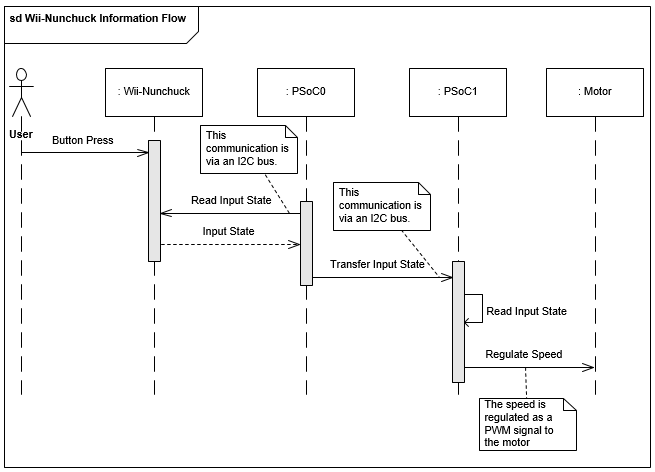
\includegraphics[width=\textwidth]{Systemarkitektur/images/WiiNunchuckSequenceDiagram.png}
	\caption{Overordnet sekvensdiagram for Wii-Nunchuck informations flow}
	\label{fig:WiiNunchuckSequenceDiagram}
\end{figure}

\subsubsection{Applikationsmodel for Nunchuck Polling Software}

\begin{figure}[H]
	\centering
	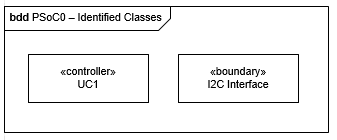
\includegraphics[scale=0.8]{Systemarkitektur/images/klasseIdentificationUC1PSoC0}
	\caption{Klasseidentifikation for PSoC0}
	\label{fig:klasseidentifikationUC1PSoC0}
\end{figure}

På figur \ref{fig:klasseidentifikationUC1PSoC0} ses klasse identifikation for Nunchuck Polling Software. Der er til Nunchuck Polling Software for Use Case 1 identificeret to klasser: \textit{UC1} samt \textit{I2C Interface}. \newline

\noindent Klassen \textit{UC1} er en controller. Dette er klassen der har til ansvar at eksekvere funktionalitet relevant til use case 1. \textit{I2C Interface} er en boundary klasse der repræsenterer grænseflade til I2C bussen.

Det kan på sekvensdiagrammet, figur \ref{fig:sekvensUC1PSoC0}, ses hvordan klasserne interagerer med hinanden. Her kan det ses at klassen \textit{UC1} aflæser Nunchuck input og herefter dekoder det, kalibrerer det, og sender det videre ud på I2C bussen hvor andre slaver kan gøre brug af dataen.

\begin{figure}[H]
	\centering
	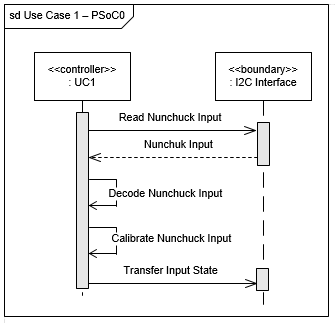
\includegraphics[scale=0.8]{Systemarkitektur/images/UC1PSoC0SequenceDiagram}
	\caption{Sekvensdiagram for PSoC0}
	\label{fig:sekvensUC1PSoC0}
\end{figure}

Figur \ref{fig:klasseUC1PSoC0} viser et endeligt klassediagram, hvor metoderne er udledt fra sekvensdiagrammet, figur \ref{fig:sekvensUC1PSoC0}. Her er det identificeret at controller klassen \textit{UC1} har to metoder til at kunne dekode og kalibrere Nunchuck data. \textit{UC1} gør brug af \textit{I2C Interface} som grænseflade til at sende dataen ud på I2C bussen.

\begin{figure}[H]
	\centering
	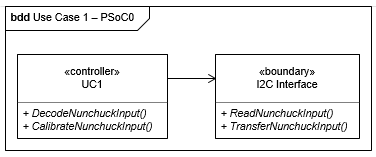
\includegraphics[scale=0.8]{Systemarkitektur/images/klasseUC1PSoC0}
	\caption{Klassediagram for PSoC0}
	\label{fig:klasseUC1PSoC0}
\end{figure}

\subsubsection{Applikationsmodel for Motor Control Software}

\begin{figure}[H]
	\centering
	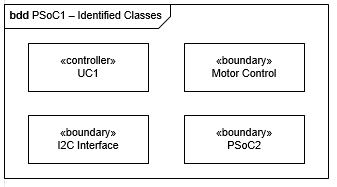
\includegraphics[scale=0.8]{Systemarkitektur/images/klasseIdentificationUC1PSoC1}
	\caption{Klasseidentifikation for PSoC1}
	\label{fig:klasseidentifikationUC1PSoC1}
\end{figure}

På figur \ref{fig:klasseidentifikationUC1PSoC1} ses klasse identifikation for Motor Control Software. Der er til Motor Control Software for Use Case 1 identificeret fire klasser: \textit{UC1}, \textit{Motor Control}, \textit{I2C Interface} og \textit{PSoC2}. \newline

\noindent \textit{UC1} er en controller. Denne klasse har til ansvar at eksekvere funktionalitet relevant til use case 1. \textit{Motor Control} repræsenterer grænsefladen til motorstyringen. \textit{I2C Interface} repræsenterer grænsefladen til I2C bussen. \textit{PSoC2} repræsenterer en grænseflade til PSoC2.

På figur \ref{fig:sekvensUC1PSoC1} ses et sekvensdiagram af interaktionen mellem disse klasser. Her kan det ses at \textit{UC1} klassen læser input data fra Nunchuck og videresender det til motor styringen samt PSoC2, så farten af motoren kan regulares og affyringsmekanismen kan aktiveres.

\begin{figure}[H]
	\centering
	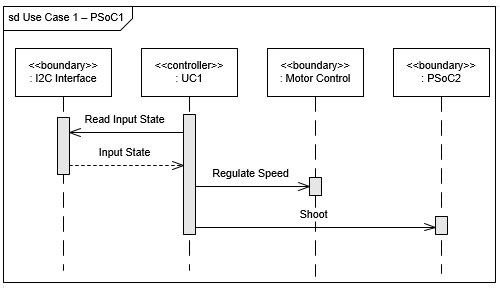
\includegraphics[scale=0.8]{Systemarkitektur/images/UC1PSoC1SequenceDiagram}
	\caption{Sekvensdiagram for PSoC1}
	\label{fig:sekvensUC1PSoC1}
\end{figure}

På figur \ref{fig:klasseUC1PSoC1} ses et endeligt klassediagram, hvor metoderne er udledt fra sekvensdiagrammet, figur \ref{fig:sekvensUC1PSoC1}. Her er det identificeret at controller klassen \textit{UC1} har primært kommunikerer med grænsefladerne \textit{I2C Interface}, \textit{PSoC2} og \textit{Motor Control}. Her skal \textit{UC1} kunne læse Nunchuck input fra \textit{I2C Interface}. Yderligere skal den kunne regulere farten på \textit{Motor Control} og affyre affyringsmekanismen.

\begin{figure}[H]
	\centering
	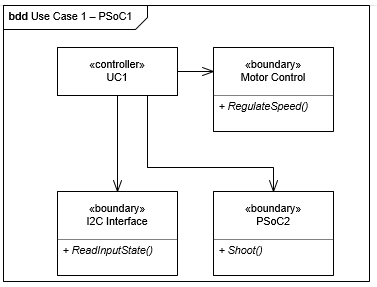
\includegraphics[scale=0.8]{Systemarkitektur/images/klasseUC1PSoC1}
	\caption{Klassediagram for PSoC1}
	\label{fig:klasseUC1PSoC1}
\end{figure}

\subsubsection{Applikationsmodel for Projectile Launcher Software}

\begin{figure}[H]
	\centering
	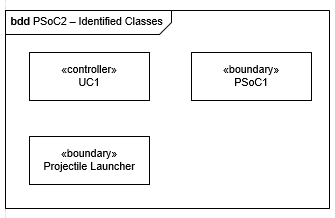
\includegraphics[scale=0.8]{Systemarkitektur/images/klasseIdentificationUC1PSoC2}
	\caption{Klasseidentifikation for PSoC2}
	\label{fig:klasseidentifikationUC1PSoC2}
\end{figure}

På figur \ref{fig:klasseidentifikationUC1PSoC2} ses klasse identifikation for Projectile Launcher Software. Der er til Projectile Launcher Software for use case 1 identificeret tre klasser: \textit{UC1}, \textit{PSoC1}, 

\begin{figure}[H]
	\centering
	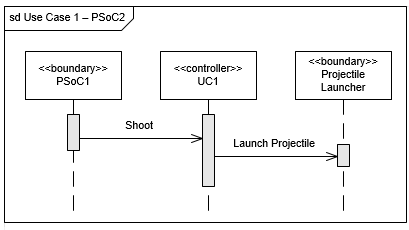
\includegraphics[scale=0.8]{Systemarkitektur/images/UC1PSoC2SequenceDiagram}
	\caption{Sekvensdiagram for PSoC2}
	\label{fig:sekvensUC1PSoC2}
\end{figure}

\begin{figure}[H]
	\centering
	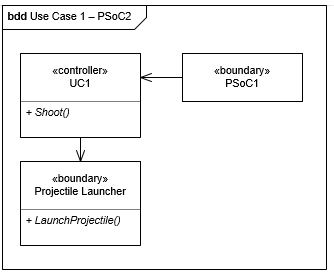
\includegraphics[scale=0.8]{Systemarkitektur/images/klasseUC1PSoC2}
	\caption{Klassediagram for PSoC2}
	\label{fig:klasseUC1PSoC2}
\end{figure}

\newpage
\subsection{Use Case 2 - Test Kommunikationsprotokoller}

Følgende afsnit præsenterer applikationsmodeller relevante til Use Case 2 - Test Kommunikationsprotokoller, fordelt over systemets CPU'er.

På figur \ref{fig:SystemTestOverviewSequenceDiagram} ses et overordnet sekvensdiagram for use casen. Her starter brugeren testen gennem brugergrænsefladen. Først bliver SPI bussen mellem DevKit8000 og PSoC0 testet. Herefter bliver I2C bussen testet ved at PSoC0 undersøger om de nødvændige I2C slaver (PSoC1 og Wii-Nunchuck) kan kommunikeres med. Til slut får brugeren en besked om at skulle trykke på en Wii-Nunchuck knap, hvorefter der bliver testet om knaptrykket skete eller ej.

\begin{figure}[H]
	\centering
	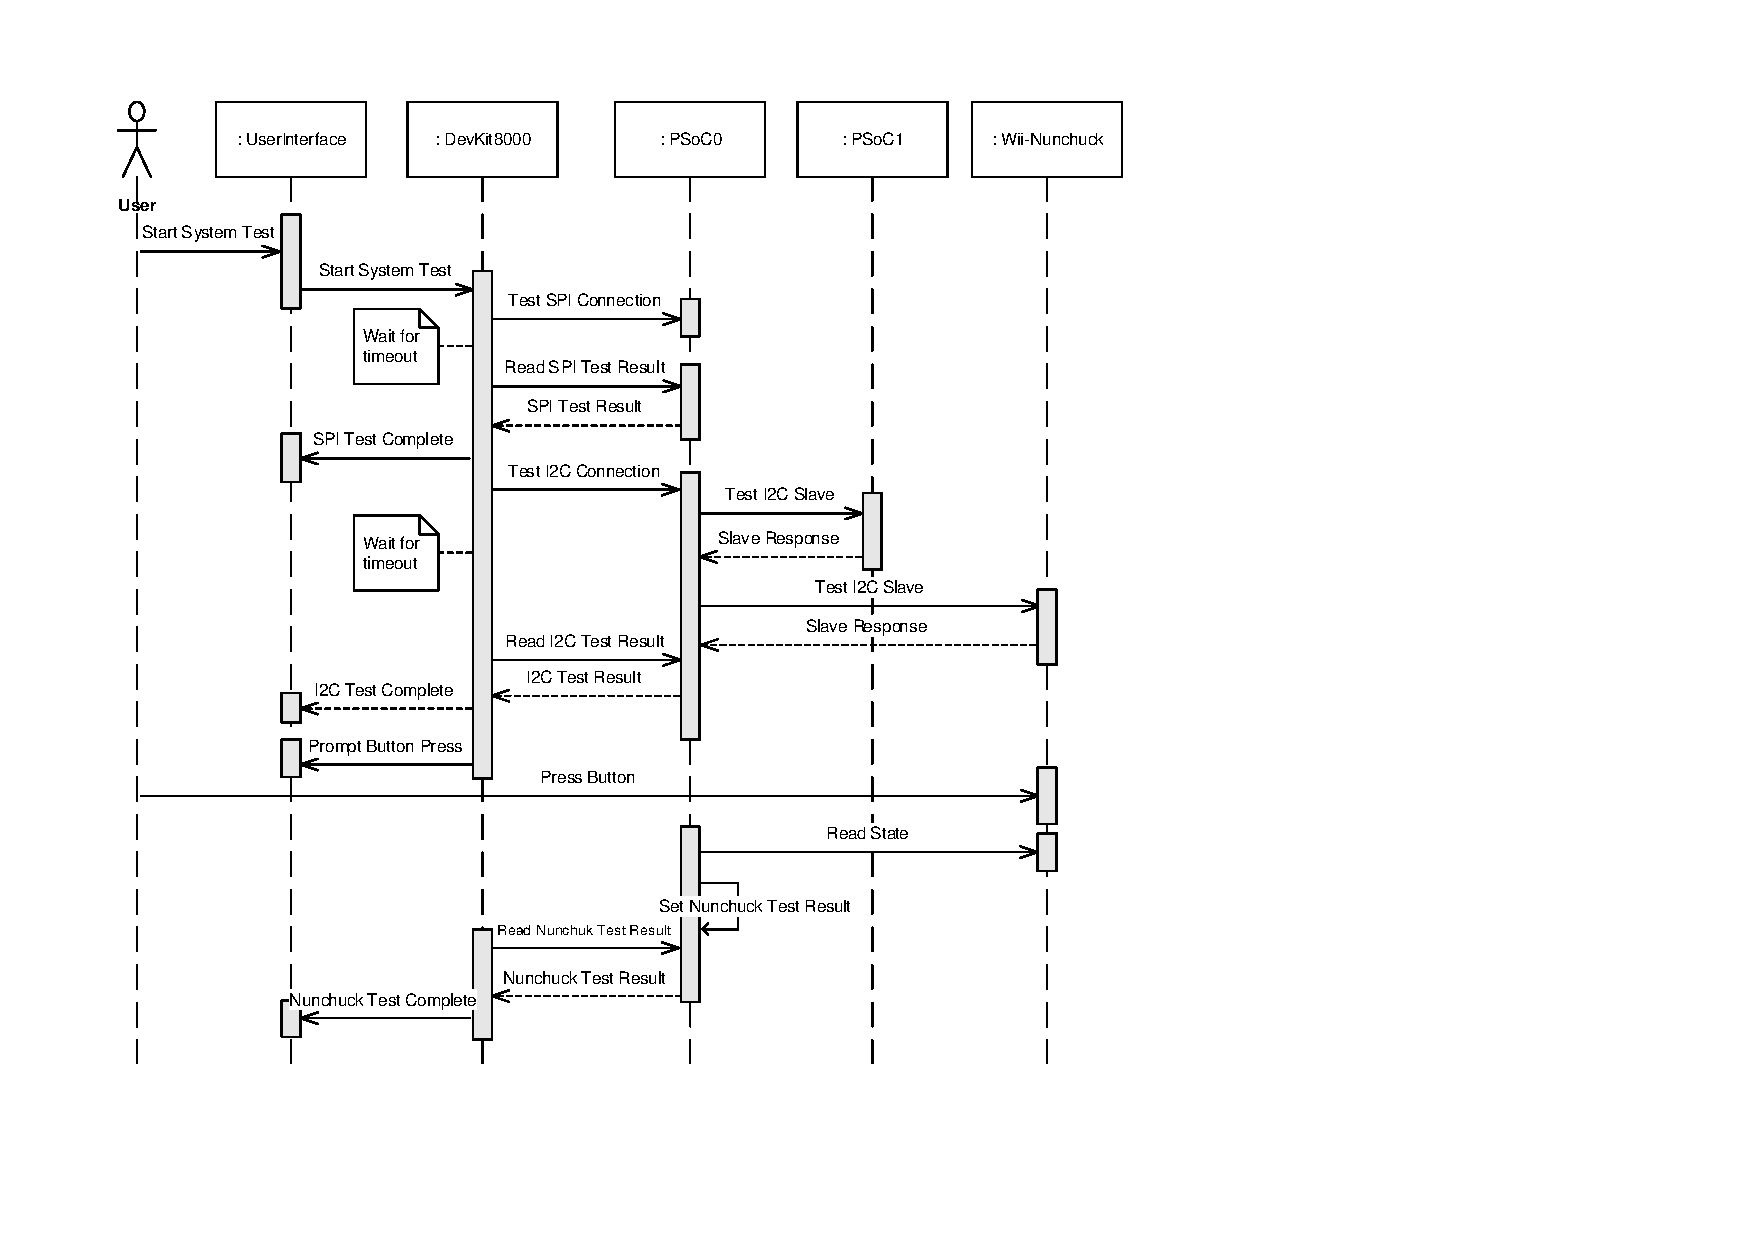
\includegraphics[width=\textwidth]{Systemarkitektur/images/OverordnetSekvensDiagramSystemTest}
	\caption{Sekvensdiagram for Use Case 2 - Test Kommunikationsprotokoller}
	\label{fig:SystemTestOverviewSequenceDiagram}
\end{figure}

% ---------------Devkit Applikationsmodel-----------------------------
\subsubsection{Applikationsmodel for User Interface Software}

\begin{figure}[H]
	\centering
	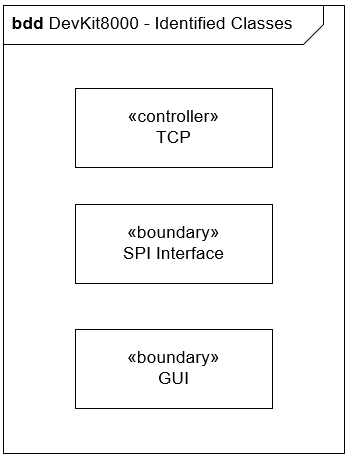
\includegraphics[scale=0.8]{Systemarkitektur/images/KlasseIdentifikationDevKit.png}
	\caption{Klasseidentifikation for Devkit 8000}
	\label{fig:klasseidentifikationDevKit}
\end{figure}

Sekvensdiagrammet for Devkit 8000 ses på figur \ref{fig:sekvensDevkit}. Kontrolklassen, som er klassen der skal udføre Use Casen, kaldes Test Communication Protocol (TCP). Der er to boundaryklasser, da DevKit 8000 skal håndtere kommunikationen med en brugergrænseflade, samt en SPI bus. Som det fremkommer af diagrammet er det kontrolklassen, der sørger for, at de forskellige tests bliver sat i gang ved at kommunikere med PSoC0 over SPI bussen. Når en test er færdiggjort meldes resultatet ud til brugeren via GUI'en.

\begin{figure}[H]
	\centering
	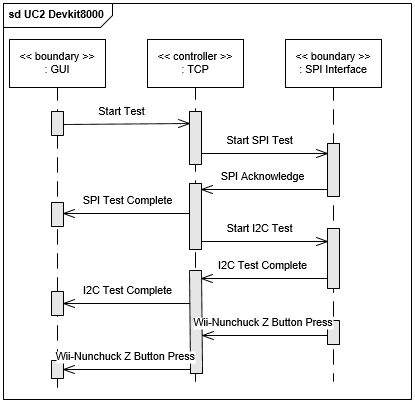
\includegraphics[]{Systemarkitektur/images/DevKit8000SequenceDiagram.png}
	\caption{Sekvensdiagram for Devkit 8000}
	\label{fig:sekvensDevkit}
\end{figure}

Ud fra sekvensdiagrammet for Devkit 8000 er der udledt metoder til klasserne. De udledte metoder ses i klassediagrammet på figur \ref{fig:klasseDevkit}. 

\begin{figure}[H]
	\centering
	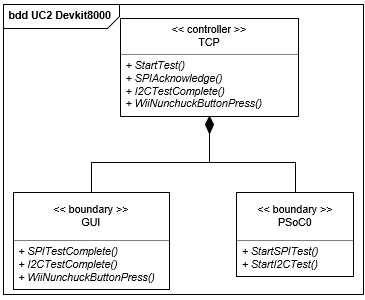
\includegraphics[] {Systemarkitektur/images/DevKit8000ClassDiagram}
	\caption{Klassediagram for Devkit 8000}
	\label{fig:klasseDevkit}
\end{figure}

% ---------------PSoC0 Applikationsmodel-----------------------------
\subsubsection{Applikationsmodel for Nunchuck Polling Software}

\begin{figure}[H]
	\centering
	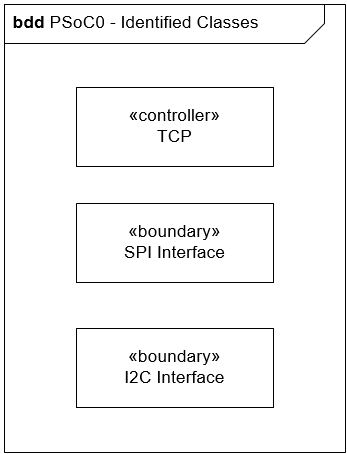
\includegraphics[scale=0.8]{Systemarkitektur/images/KlasseIdentifikationPSoC0.png}
	\caption{Klasseidentifikation for PSoC0}
	\label{fig:klasseidentifikationPSoC}
\end{figure}

På figur \ref{fig:sekvensPSoC0SPITest}, \ref{fig:sekvensPSoC0I2CTest} og \ref{fig:sekvensPSoC0NunchuckTest} ses sekvensdiagrammer for PSoC0. Sekvensdiagrammerne er blevet opdelt i de 3 tests der gennemføres i use casen; SPI, I2C og Nunchuck kommunikations tests. Kontrolklassen er Test Communication Protocol, hvilket på figurerne er forkortet til TCP. Derudover er der tre boundaryklasser, da PSoC0 skal kommunikere både med Devkit 8000, Nunchucken og PSoC1.

\begin{figure}[H]
	\centering
	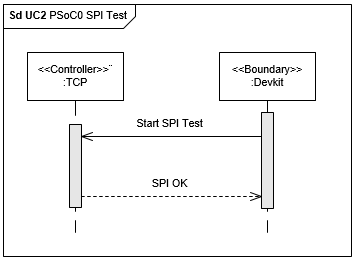
\includegraphics[width=.8\textwidth] {Systemarkitektur/images/SDPSoC0SPITest}
	\caption{Sekvensdiagram for PSoC0 SPI test}
	\label{fig:sekvensPSoC0SPITest}
\end{figure}

På figur \ref{fig:sekvensPSoC0SPITest} ses, at Devkittet sender en besked til kontrolklassen for at påbegynde SPI testen. Når testen er udført, svarer denne med en SPI OK og derved er SPI testen gennemført.

\begin{figure}[H]
	\centering
	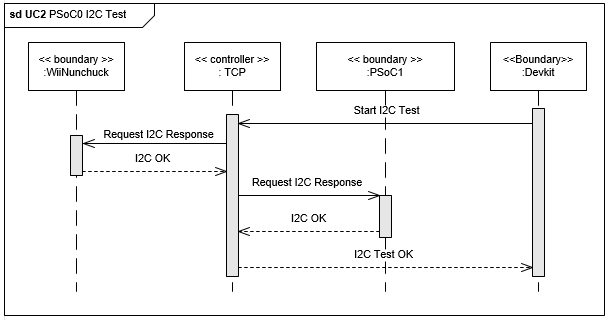
\includegraphics[width=\textwidth] {Systemarkitektur/images/SDPSoC0I2CTest}
	\caption{Sekvensdiagram for PSoC0 I2C test}
	\label{fig:sekvensPSoC0I2CTest}
\end{figure}

På figur \ref{fig:sekvensPSoC0I2CTest} ses, at Devkittet starter I2C testen, ved at sende en besked til kontrolklassen. Kontrolklassen anmoder herefter om svar via I2C nettet fra Nuchucken og PSoC1. Når disse enheder har svaret med et I2C OK er testen gennemført og der sendes besked til Devkittet med en I2C Test OK.

\begin{figure}[H]
	\centering
	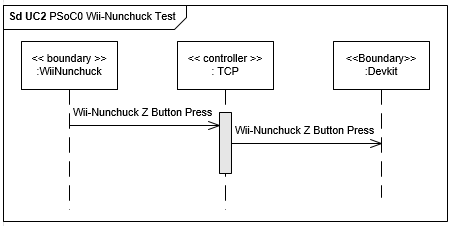
\includegraphics[width=\textwidth] {Systemarkitektur/images/SDPSoC0NunchuckTest}
	\caption{Sekvensdiagram for PSoC0 Nunchuck test}
	\label{fig:sekvensPSoC0NunchuckTest}
\end{figure}

På figur \ref{fig:sekvensPSoC0NunchuckTest} ses sekvensdiagrammet for Wii-Nunchuck testen. Når der sker et tryk sender Nunchucken 'Z' knappens status til kontrolklassen. Herefter videresender kontrolklassen knappens status til Devkittet og derved er testen færdig.\newline

\begin{figure}[H]
	\centering
	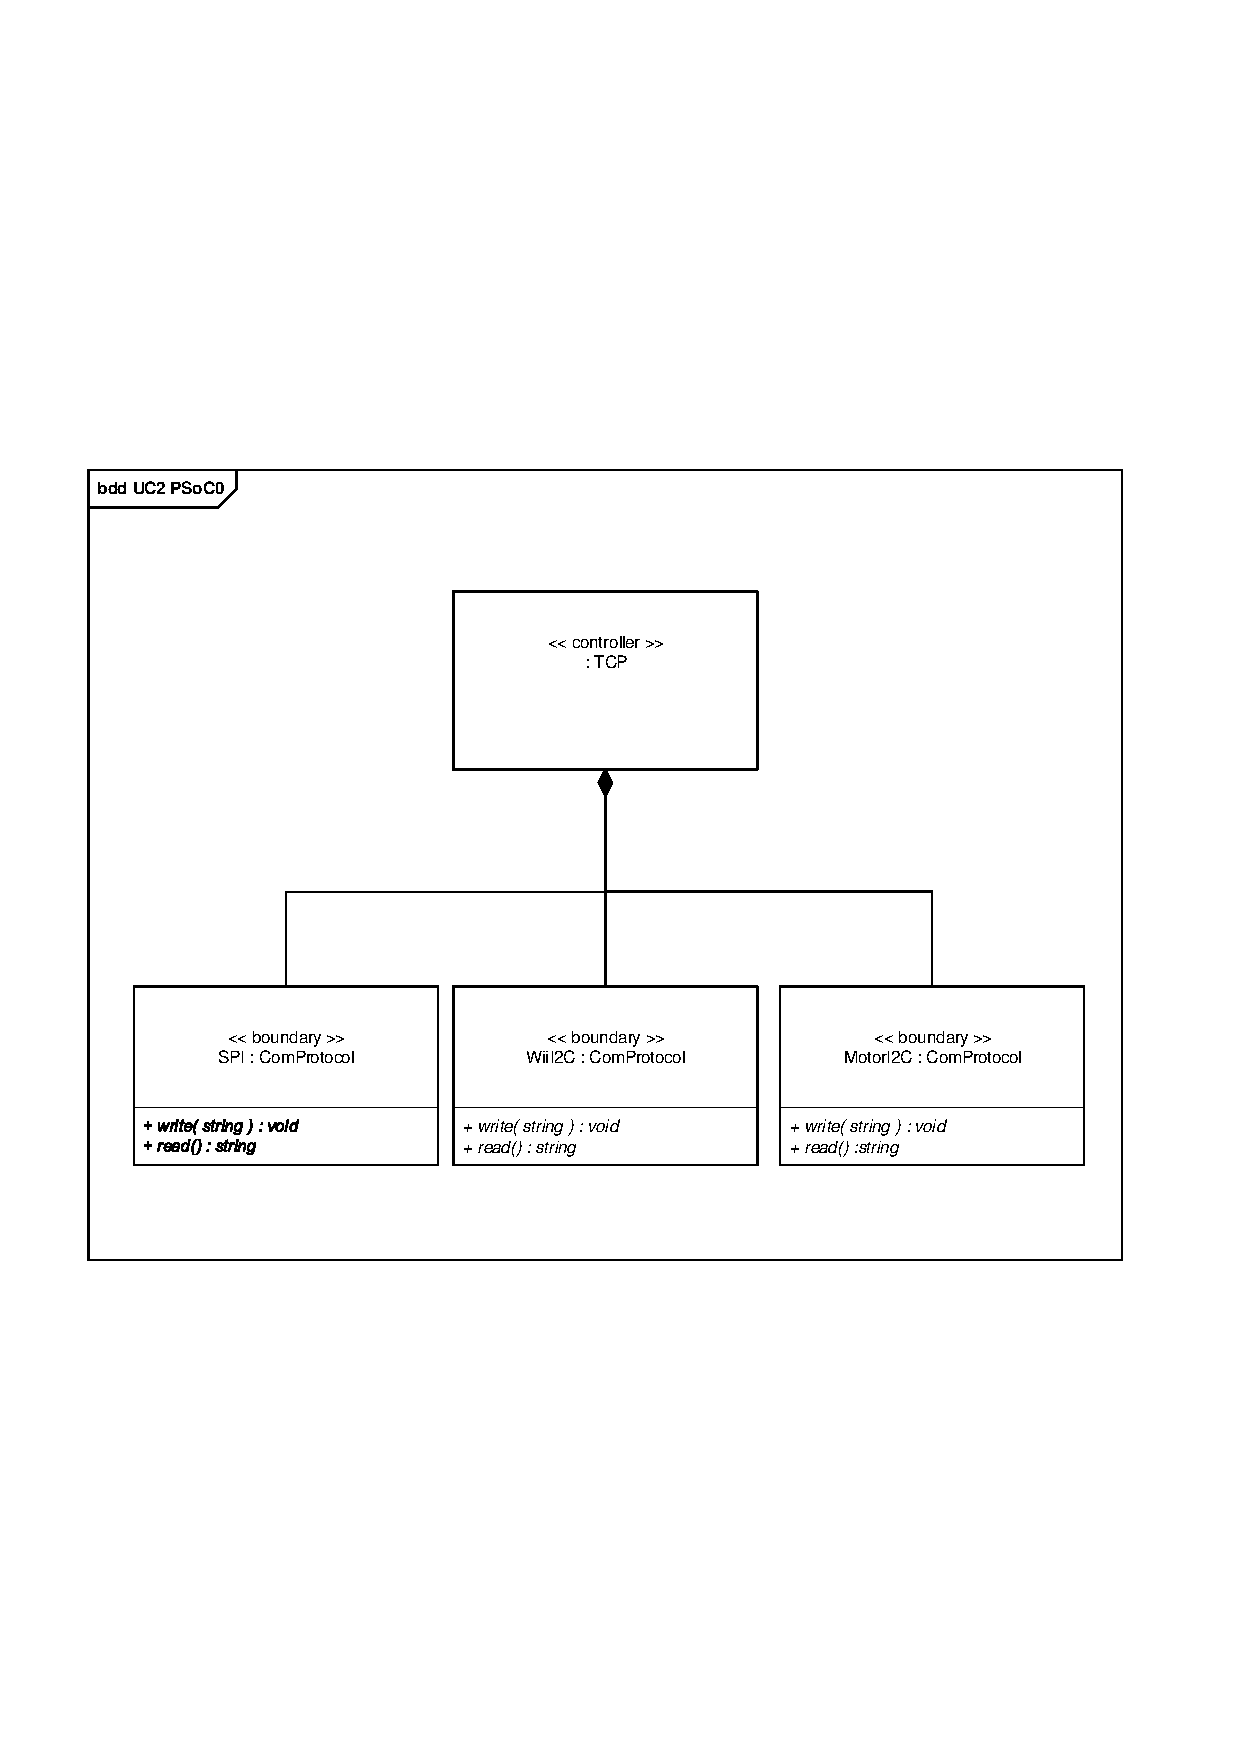
\includegraphics[width=\textwidth]{Systemarkitektur/images/klassediagramPSoC0}
	\caption{Klassediagram for PSoC0}
	\label{fig:klassePSoC0}
\end{figure}

I klassediagrammet på figur \ref{fig:klassePSoC0} ses kontrolklassen og de tre boundaryklasser, som hører til PSoC0. I klasserne er der tilføjet metoder, som er udledt ud fra sekvensdiagrammerne. 

% ---------------PSoC1 Applikationsmodel-----------------------------
\subsubsection{Applikationsmodel for Motor Control Software}

\begin{figure}[H]
	\centering
	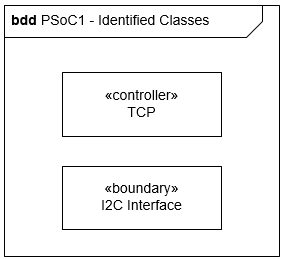
\includegraphics[scale=0.8]{Systemarkitektur/images/KlasseIdentifikationPSoC1.png}
	\caption{Klasseidentifikation for PSoC1}
	\label{fig:klasseidentifikationPSoC1}
\end{figure}

Sekvensdiagrammet for PSoC1 ses på figur \ref{fig:sekvensPSoC1I2CTest}. Som forrig afsnit er kontrolklassen Test Communication Protocols, hvilket i diagrammet er forkortet til TCP. I dette tilfælde er der kun én boundaryklasse, da PSoC1, i denne use case, kun anvendes til I2C testen og derfor kun skal kommunikere med PSoC0. 

\begin{figure}[H]
	\centering
	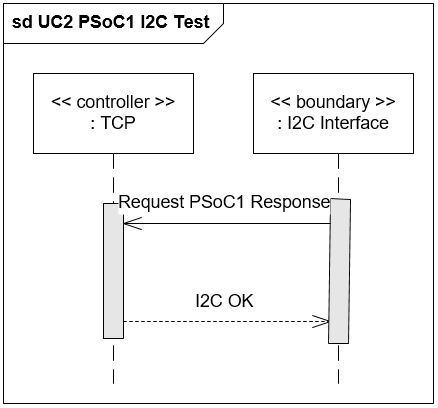
\includegraphics[width=.8\textwidth] {Systemarkitektur/images/SDPSoC1I2CTest}
	\caption{Sekvensdiagram for PSoC1}
	\label{fig:sekvensPSoC1I2CTest}
\end{figure}

På figur \ref{fig:sekvensPSoC1I2CTest} ses, at boundaryklassen, PSoC0, anmoder om respons fra kontrolklassen til at bekræfte om at I2C slaven kan kommunikeres med. Hvis dette er tilfældet sendes der I2C OK tilbage til boundaryklassen.  

\begin{figure}[H]
	\centering
	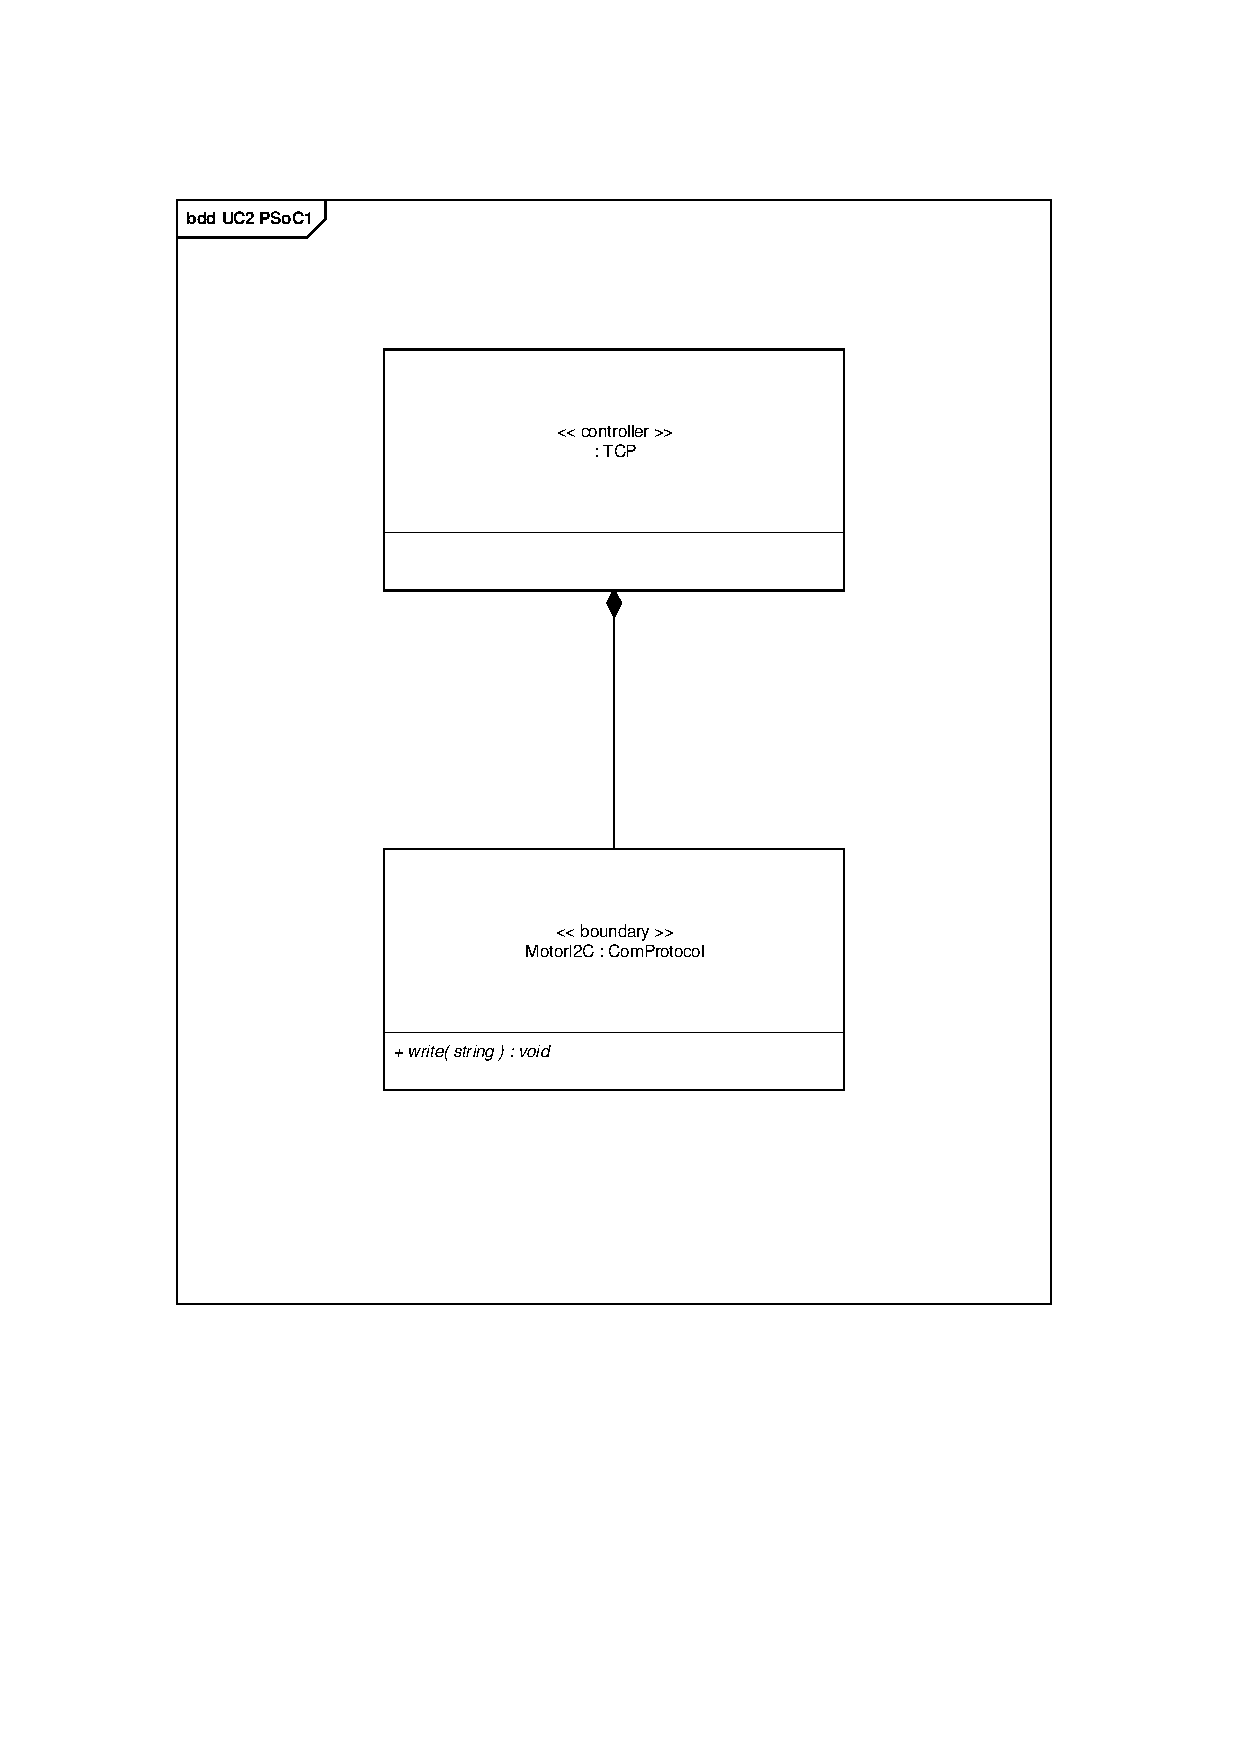
\includegraphics[width=.5\textwidth]{Systemarkitektur/images/klassediagramPSoC1}
	\caption{Klassediagram for PSoC1}
	\label{fig:klassePSoC1}
\end{figure}

Fra sekvensdiagrammet på figur \ref{fig:sekvensPSoC1I2CTest} udledes et klassediagram som ses foroven i figur \ref{fig:klassePSoC1}.

\section{Samlede Klassediagrammer}
På af de detaljerede applikationsmodeller for use case 1- og 2, er der udledt samlede klassediagrammer for hver individuel CPU i systemet. Disse er med til at identificere konceptuelle klasser og funktionaliter der skal overvejes i implementation og design af systemet, og har altså fungeret som et udgangspunkt til resten af udviklingsprocessen.\newline\noindent
Figur \ref{fig:CompleteClassDiagramDevKit8000}, \ref{fig:CompleteClassDiagramPSoC0}, \ref{fig:CompleteClassDiagramPSoC1}, og \ref{fig:CompleteClassDiagramPSoC2} vises de samlede klassediagrammer for hver CPU.\newline\noindent
For disse klassediagrammer er der konceptuelle klasser som gentager sig selv. Alle klassediagrammer har én klasse af typen \textit{controller}. Disse klasse indeholder alt funktionalitet der er nødvændig for at kunne implementere systemets Use Cases. Yderligere bliver klasserne \textit{I2C Interface} samt \textit{SPI Interface} gentaget. Disse repræsenterer klasser for de tilsvarende bustyper, I2C og SPI, og bruges af softwaren til at sende og modtage data på disse busser.\newline\noindent
På figur \ref{fig:CompleteClassDiagramDevKit8000} ses det at DevKit8000 controlleren skal have funktionalitet til start af system test, i relation til Use Case 2. For at kunne udføre dette kommunikerer den med grænsefladen Graphical User Interface (\textit{GUI}), for at kunne vise resultater til brugeren. Desuden skal controlleren kommunikere med grænsefladen \textit{SPI Interface}, for at sende data ud til til resten af systemet via SPI bussen.

\begin{figure}[H]
	\centering
	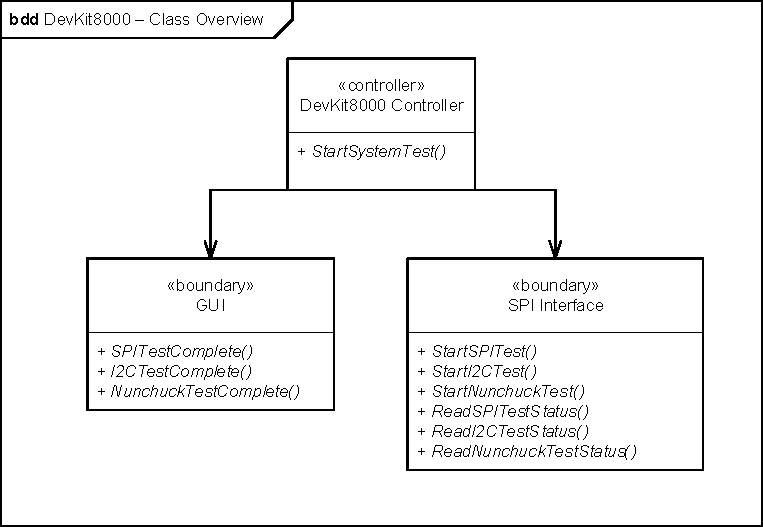
\includegraphics[width=\textwidth] {Systemarkitektur/images/CompleteClassDiagramDevKit8000}
	\caption{Samlet Klassediagram for DevKit8000}
	\label{fig:CompleteClassDiagramDevKit8000}
\end{figure}

På figur \ref{fig:CompleteClassDiagramPSoC0} ses det at PSoC0 controlleren skal have funktionalitet til at starte tests af systemets busser. Yderligere skal den også kunne dekode og kalibrere data der kommer fra Nunchuck. I relation til disse funktionaliteter skal den kunne modtage og sende data på systemets I2C og SPI busser.

\begin{figure}[H]
	\centering
	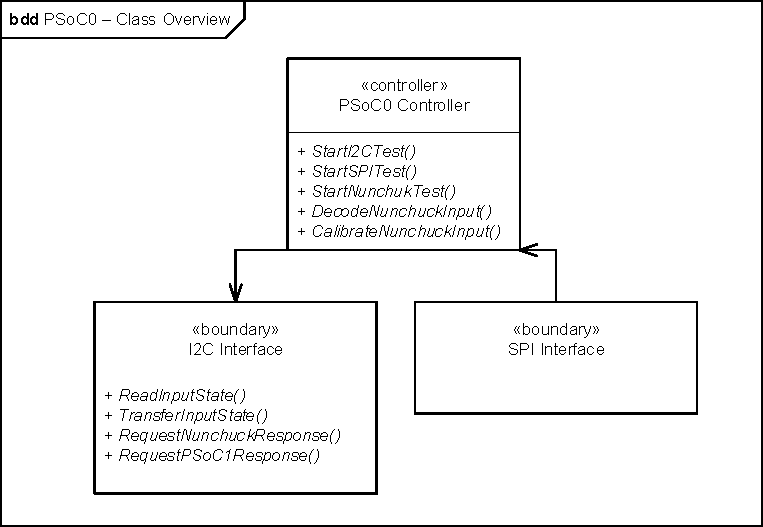
\includegraphics[width=\textwidth] {Systemarkitektur/images/CompleteClassDiagramPSoC0}
	\caption{Samlet Klassediagram for PSoC0}
	\label{fig:CompleteClassDiagramPSoC0}
\end{figure}

På figur \ref{fig:CompleteClassDiagramPSoC1} ses det at PSoC1 controlleren kommunikerer med grænsefladerne \textit{I2C Interface}, \textit{Motor Control} samt \textit{PSoC2}. Controlleren skal kunne regulere fart på systemets motorstyring, for at kunne styre kanonen. Desuden skal den kunne sende en affyringsbesked til \textit{PSoC2}. For at regulere fart og affyre kanonen, skal controlleren kunne aflæse Nunchucken's tilstand fra \textit{I2C Interface}.
\begin{figure}[H]
	\centering
	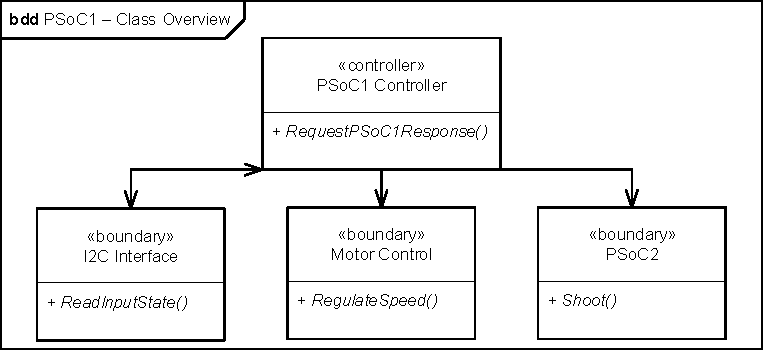
\includegraphics[width=\textwidth] {Systemarkitektur/images/CompleteClassDiagramPSoC1}
	\caption{Samlet Klassediagram for PSoC1}
	\label{fig:CompleteClassDiagramPSoC1}
\end{figure}

På figur \ref{fig:CompleteClassDiagramPSoC2} ses det at PSoC2 skal have funktionalitet til at aktivere afskydning, som gøres ved at kommunikere med grænsefladen \textit{Projectile Launcher}. Afskydningen aktiveres af grænsefladen \textit{PSoC1}.
\begin{figure}[H]
	\centering
	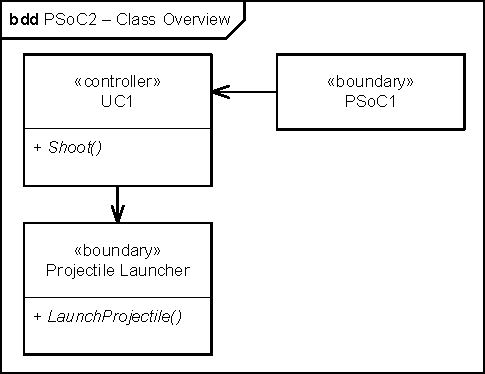
\includegraphics[width=\textwidth] {Systemarkitektur/images/CompleteClassDiagramPSoC2}
	\caption{Samlet Klassediagram for PSoC2}
	\label{fig:CompleteClassDiagramPSoC2}
\end{figure}

\section{Kommunikationsprotokoller}
\label{afsnit:kommunikationsprotokoller}
I dette afsnit beskrives de kommunikationsprotokoller der anvendes til at sende data mellem systemets komponenter på de anvendte bustyper - I2C og SPI. På figur \ref{fig:kommunikationsOverblik} ses hvilke bustyper der anvendes mellem systemets komponenter. 

\begin{figure}[H]
	\centering
	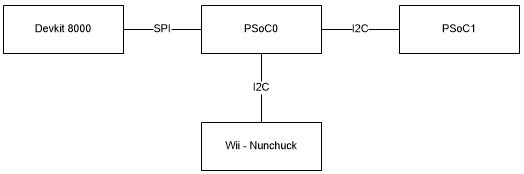
\includegraphics[width=\textwidth] {Systemarkitektur/images/anvendtebustyper}
	\caption{Forbindelser mellem systemets komponenter}
	\label{fig:kommunikationsOverblik}
\end{figure}

\subsection{SPI Protokol}
\label{afsnit:spiprotokol}
Til kommunikation mellem Devkittet og PSoC0 anvendes der \textit{Serial Parallel Interface (SPI)}. SPI-forbindelsen består af fire signaler. Et af signalerne er \textit{slave select} (SS). Det muliggør kommunikation med flere slaver. Selve dataen sendes via signalerne \textit{Master Out Slave In} (MOSI) og \textit{Master In Slave Out} (MISO). Det foregår ved \textit{Full Duplex}, hvor der altid sendes i begge retninger på én gang. Hvis der kun ønskes at sende i én retning, kan der sendes 0'er i den anden retning. Derudover er der en \textit{Clock} (SCLK), som sørger for at kommunikationen er synkron. I forhold til timing er det vigtigt, at både master og slave anvender samme \textit{Timing Mode}, som styres af to bit, \textit{SPI Clock Polarity Bit} (CPOL), som bestemmer om clock'en starter højt eller lavt, og \textit{SPI Clock Phase Bit} (CPHA), som afgør om data samples på clock'ens rising- eller falling edge. I dette projekt anvendes \textit{Timing Mode 3}, hvor clock'en starter høj og sampler på rising edge. \\
De kommandoer, der i projektet sendes via SPI, består af 8 bit. \\
På tabel \ref{tabel:spiKommandoType} ses SPI-protokollen. Til venstre på tabellen ses navnet på de kommandoer, der sendes. Alle kommandoer med "TEST" i navnet sendes fra Devkit8000 til PSoC0 via MOSI. De resterende kommandoer er svar på de forskellige tests, som sendes via MISO fra PSoC0 til Devkit8000. Det er værd at lægge mærke til, at det er bevidst, at der ikke er en kommando for SPI\_FAIL. Da SPI-forbindelsen ikke testes på PSoC0, men ved at PSoC0 sender \textit{SPI\_OK} tilbage til Devkit8000 via SPI-forbindelsen. Dermed kan det først afgøres om SPI-forbindelsen fungerer korrekt, når Devkit8000, modtager (eller ikke modtager) succes-beskeden fra PSoC0. \\


\begin{table}[H]
	\centering
	\resizebox{\textwidth}{!}{%
		\begin{tabular}{llll}
			\hline
			\multicolumn{1}{|l|}{Kommandotype}                                & \multicolumn{1}{l|}{Beskrivelse}                        & \multicolumn{1}{l|}{Binær Værdi} & \multicolumn{1}{l|}{Hex Værdi} \\ \hline
			\rowcolor[HTML]{CBCEFB} 
			{\color[HTML]{000000} START\_SPI\_TEST}                           & {\color[HTML]{000000} Sætter PSoC0 i 'SPI-TEST' mode}   & 1111 0001                        & 0xF1                           \\
			START\_I2C\_TEST                                                  & Sætter PSoC0 i 'I2C-TEST' mode                          & 1111 0010                        & 0xF2                           \\
			\rowcolor[HTML]{CBCEFB} 
			\begin{tabular}[c]{@{}l@{}}START\_NUN-\\ CHUCK\_TEST\end{tabular} & Sætter PSoC0 i 'NUNCHUCK-TEST' mode                     & 1111 0011                        & 0xF3                           \\
			SPI\_OK                                                           & Signalerer at SPI-testen blev gennemført uden fejl      & 1101 0001                        & 0xD1                           \\
			\rowcolor[HTML]{CBCEFB} 
			I2C\_OK                                                           & Signalerer at I2C-testen blev gennemført uden fejl      & 1101 0010                        & 0xD2                           \\
			I2C\_FAIL                                                         & Signalerer at der skete fejl under I2C-testen           & 1100 0010                        & 0xC2                           \\
			\rowcolor[HTML]{CBCEFB} 
			NUNCHUCK\_OK                                                      & Signalerer at NUNCHUCK-testen blev gennemført uden fejl & 1101 0011                        & 0xD3                           \\
			NUNCHUCK\_FAIL                                                    & Signalerer at der skete fejl under NUNCHUCK-testen      & 1100 0011                        & 0xC3                          
		\end{tabular}
	}
	\caption{Kommandotyper der anvendes ved SPI kommunikation}
	\label{tabel:spiKommandoType}
\end{table}

For at aflæse en besked fra SPI-slaven, skal slaven først klargøre dens SPI-transfer buffer. Dette gøres ved, at SPI-masteren sender en commandotype til slaven, som derefter tolker kommandotypen, og eksekverer kommandoen, hvor SPI-transfer bufferen bliver sat. Imens dette sker, venter SPI-masteren i et bestemt stykke tid, for at sikre at transfer-bufferen når at blive sat. På figur \ref{figure:SDSpiReadSlave} ses et sekvensdiagram der illustrerer dette. 

\begin{figure}[H]
	\centering
	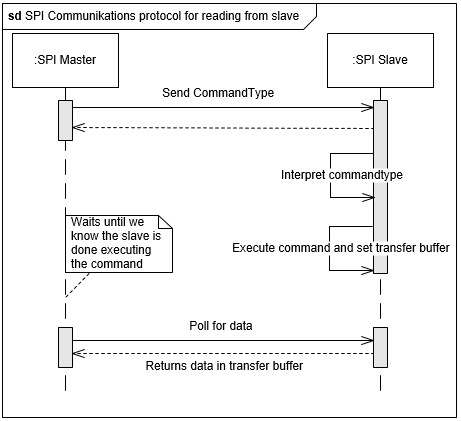
\includegraphics[]{SystemArkitektur/images/SDSpiSlaveRead}
	\caption{Sekvensdiagram for at læse fra SPI-slaven}
	\label{figure:SDSpiReadSlave}
\end{figure}


\subsection{I2C Protokol}
\label{afsnit:I2CProtokol}

I2C\cite{I2C} er en bus bestående af to ledninger. Den ene ledning bruges som databus og navngives \textit{Serial Data Line} (SDA). Den anden ledning bruges til clock signalet, der synkroniserer kommunikationen, og navngives \textit{Serial Clock Line} (SCL). Enheder på I2C bussen gør brug af et master-slave forhold til at sende og læse data. En fordel ved I2C bussen er at netværket kan bestå af multiple masters og slaver, hvilket udnyttes i dette system da tre I2C komponenter skal sende data mellem hinanden.

I2C gør brug af en integreret protokol der anvender adressering af hardware-enheder for at identificere hvilken enhed der kommunikeres med. På tabel \ref{table:I2CAddress} ses addresserne tildelt systemets PSoCs.

\begin{table}[H]
	\centering
	\begin{tabular}{lllllllll}
		\hline
		\multicolumn{1}{|l|}{I2C Adresse bits} & 7                        & 6                        & 5                        & 4 & 3 & 2 & \multicolumn{1}{l|}{1} & \multicolumn{1}{l|}{0 (R/W)} \\ \hline
		\rowcolor[HTML]{CBCEFB} 
		{\color[HTML]{000000} PSoC0}           & {\color[HTML]{000000} 0} & {\color[HTML]{000000} 0} & {\color[HTML]{000000} 0} & 1 & 0 & 0 & 0                      & 0/1                          \\
		PSoC1                                  & 0                        & 0                        & 0                        & 1 & 0 & 0 & 1                      & 0/1                         
	\end{tabular}
	\caption{Adresser der anvendes på I2C bussen}
	\label{table:I2CAddress}
\end{table}

Den integrerede I2C protokol sender data serielt i pakker af 8-bit (1 byte). På figur \ref{fig:I2CTimingDiagram} ses et timing diagram for aflæsning af 1 byte. Figuren er et udsnit fra databladet for en LM75, der anvender fire faste addressebits, tre vilkårlige bit og en read/write bit. Her ses at transmissionen af data begynder med en addresse-byte til slaven efterfulgt en acknowledge til masteren og herefter sendes en data-byte. 

\begin{figure}[H]
	\centering
	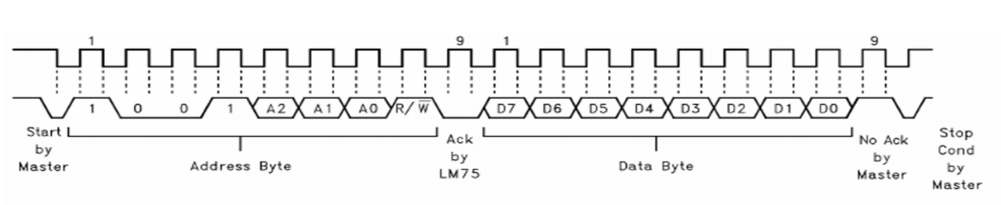
\includegraphics[width=\textwidth] {Systemarkitektur/images/I2CTimingDiagram}
	\caption{Timing Diagram af 1-byte I2C aflæsning}
	\label{fig:I2CTimingDiagram}
\end{figure}

Goofy candygun gør brug af I2C protokollen via PSoC's I2C \textit{Application Programming Interface} (API). Ved brug af denne API er der blevet udviklet en kommunikationsprotokol mellem systemets PSoCs, som gør det muligt at sende kommandoer og data.

Da I2C dataudveksling sker bytevist, er kommunikations protokollen opbygget ved, at kommandoens type indikeres af den første modtagne byte. Herefter følger \textit{N}-antal bytes som er kommandoens tilhørende data. \textit{N} er et vilkårligt heltal og bruges i dette afsnit når der refereres til en mængde data-bytes der sendes med en kommandotype.

Kommandoens type definerer antallet af databytes modtageren skal forvente og hvordan disse skal fortolkes. På figur \ref{fig:I2CProtokolEksempel} ses et sekvensdiagram der, med pseudo-kommandoer, demonstrerer forløbet mellem en I2C afsender og modtager ved brug af kommunikations protokollen.

\begin{figure}[H]
	\centering
	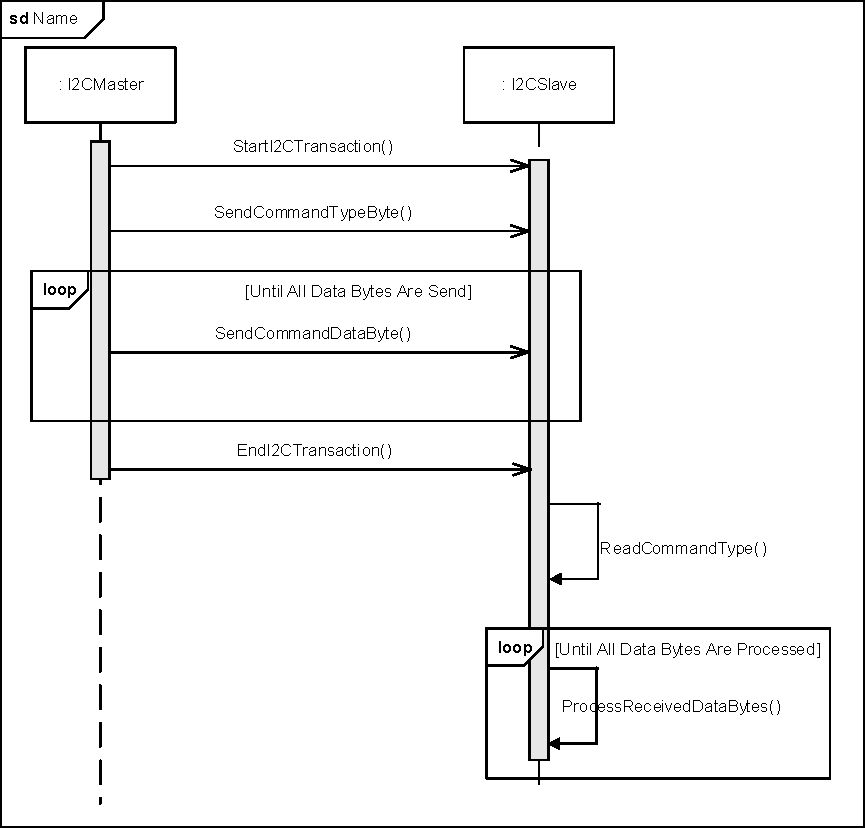
\includegraphics[width=\textwidth] {Systemarkitektur/images/I2CProtocol}
	\caption{Eksempel af I2C Protokol Forløb}
	\label{fig:I2CProtokolEksempel}
\end{figure}

På figur \ref{fig:I2CProtokolEksempel} ses at afsenderen først starter en I2C transaktion, hvorefter typen af kommando sendes som den første byte. Efterfølgende sendes \textit{N} antal bytes, afhængig af hvor meget data den givne kommandotype har brug for at sende. Efter afsluttet I2C transaktion læser I2C modtageren typen af kommando, hvor den herefter kan fortolke \textit{N} antal modtagne bytes afhængig af den modtagne kommandotype.

På tabel \ref{table:I2CKommandoer} ses de definerede kommandotyper og det tilsvarende antal af bytes der sendes ved dataveksling.

\begin{table}[H]
	\centering
	\resizebox{\textwidth}{!}{
		\begin{tabular}{lllll}
			\hline
			\multicolumn{1}{|l|}{Kommandotype}    & \multicolumn{1}{l|}{Beskrivelse}                                            & \multicolumn{1}{l|}{Binær Værdi} & \multicolumn{1}{l|}{Hex Værdi} & \multicolumn{1}{l|}{Data Bytes}                                                                                         \\ \hline
			\rowcolor[HTML]{CBCEFB} 
			{\color[HTML]{000000} NunchchuckData} & {\color[HTML]{000000} Indeholder aflæst data fra Wii Nunchuck controlleren} & 0010 1010                        & 0xA2                           & \begin{tabular}[c]{@{}l@{}}Byte \#1 Analog X-værdi\\ Byte \#2 Analog Y-værdi\\ Byte \#3 Analog Buttonstate\end{tabular} \\
			I2CTestRequest                        & Anmoder PSoC0 om at starte I2C-kommunikations test                          & 0010 1001                        & 0x29                           & Ingen databyte                                                                                                          \\
			\rowcolor[HTML]{CBCEFB} 
			I2CTestAck                            & Anmodning om at få en I2C OK besked fra I2C enhed                           & 0010 1000                        & 0x28                           & Ingen databyte                                                                                                         
		\end{tabular}
	}
	\caption{Kommandotyper der anvendes ved I2C kommunikation}
	\label{table:I2CKommandoer}
\end{table}

Kolonnerne "Binær Værdi" og "Hex Værdi" i tabel \ref{table:I2CKommandoer} viser kommandotypens unikke tal-ID i både binær- og hexadecimalform. Denne værdi sendes som den første byte, for at identificere kommandotypen. 

\section{Brugergrænseflade}


Ved hjælp af en brugergrænseflade, kan systemtesten styres fra DevKit8000.
Brugergrænsefladen er opbygget ud fra sekvensdiagrammet figur \ref{fig:SystemTestOverviewSequenceDiagram},
ud fra dette kunne brugergrænsefladen skitseres som figur \ref{fig:GUISkitse}.
Grænsefladen mellem DevKit8000 og PSoC0 er en SPI-bus som ses på figur \ref{fig:IBD}, og brugergrænsefladen er koblet til DevKit8000 ved hjælp af en interfacedriver.
Brugergrænsefladen skal sende startsekvensen til interfacedriveren, hvorefter dette sendes til PSoC0 og videre ud i systemet.
Brugergrænsefladen skal aflæse svaret fra systemtesten og printe dette ud i en konsol.

\begin{figure}[H]
	\centering
	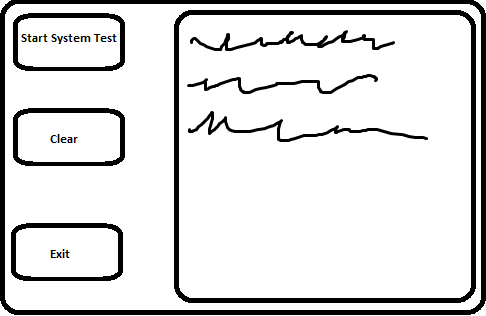
\includegraphics[width=\textwidth] {Systemarkitektur/images/GUISkitse}
	\caption{Skitse af brugergrænseflade}
	\label{fig:GUISkitse}
\end{figure}


Brugergrænsefladen er designet ud fra den sekventielle struktur i usecase 2, se afsnit \ref{afsnit:FUC2}. Dette er løst ved hjælp af Event-Driven Programming.
Denne model drives ved hjælp af events, som i dette tilfælde aktiveres af brugeren ved knaptryk. Knapperne vil blive tildelt forskellige funktionaliteter, der faciliterer systemtesten.

Et alternativ kunne være trådbaseret design. Interfacedriveren kunne oprettes som en seperat tråd fra GUI'en, der ville køre den samme funktionalitet. Dette ville være unødvendigt i forhold til den sekvetielle struktur i systemet. Kompleksiteten i dette design ville være overvældende i forhold til den ønskede funktionalitet og blev derfor fravalgt.


	\chapter{Design og Implementering}

\section{Hardware}

\subsection{Motorstyring}
\subsubsection{H-bro}
\subsubsection{Detektor}
Denne detektor består af et potentiometer og en ADC, som er en del af “motorstyring” blokken, så ved hjælp af potentiometeret kan man sørge for, at motoren ikke drejer for langt ud til begge sider.  Der kunne være brugt en stepper-motor til at styre det med, men for at få mere hardware med, blev det besluttet, at det var en bedre løsning at gøre det på denne måde.
\begin{figure}[H]
	\centering
	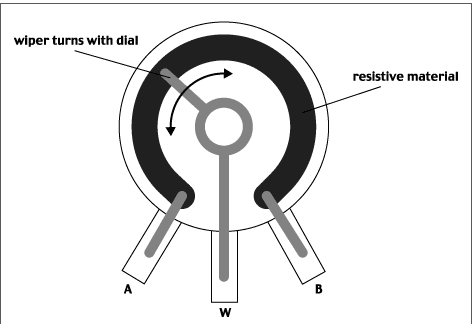
\includegraphics[width=\textwidth]{Afsnit/DesignOgImplementering/images/poten}
	\caption{potentiometer}
	\label{fig:poten}
\end{figure}
\textbf{måske et billede af opstilling i stedet for}\\
Potentiometeret har til formål at skulle holde styr på, at motoren ikke kører længere ud end det hvad det fastsatte krav er. Der er blevet valgt at bruge et Potentiometer som er et linæret et, som vil sige at når man for hver ændring man laver på Potentiometeret, vil der også ske en ændring i output spændingen. Så når den bliver fast gjord til motoren vil man kunne se en ændring i den spænding som kommer ud fra potentiometeret, som bliver sendt ind i ADC’en, som er af typen Sequencing Successive Approximation ADC, som er placeret internt i PSoC’en. Så når output spændingen fra potentiometer bliver aflæst, vil man kunne vide præcise hvor motoren er.  
ADC’en er en sample hold kreds, som vil sige den holder på dataen end til der er fundet en værdi, så der går noget tid i mellem hver værdi, så der er søgeret for at der ikke bliver lavet over samples og der ikke bliver lavet aliasing af det signal som kommer ind i ADC’en. For at finde den værdi som bliver sendt ind i ADC'en, bliver der lavet en skala som bliver halvert alt efter hvor værdien ligger på skalaen, som vist på figur \ref{fig:pot}

\begin{figure}[H]
	\centering
	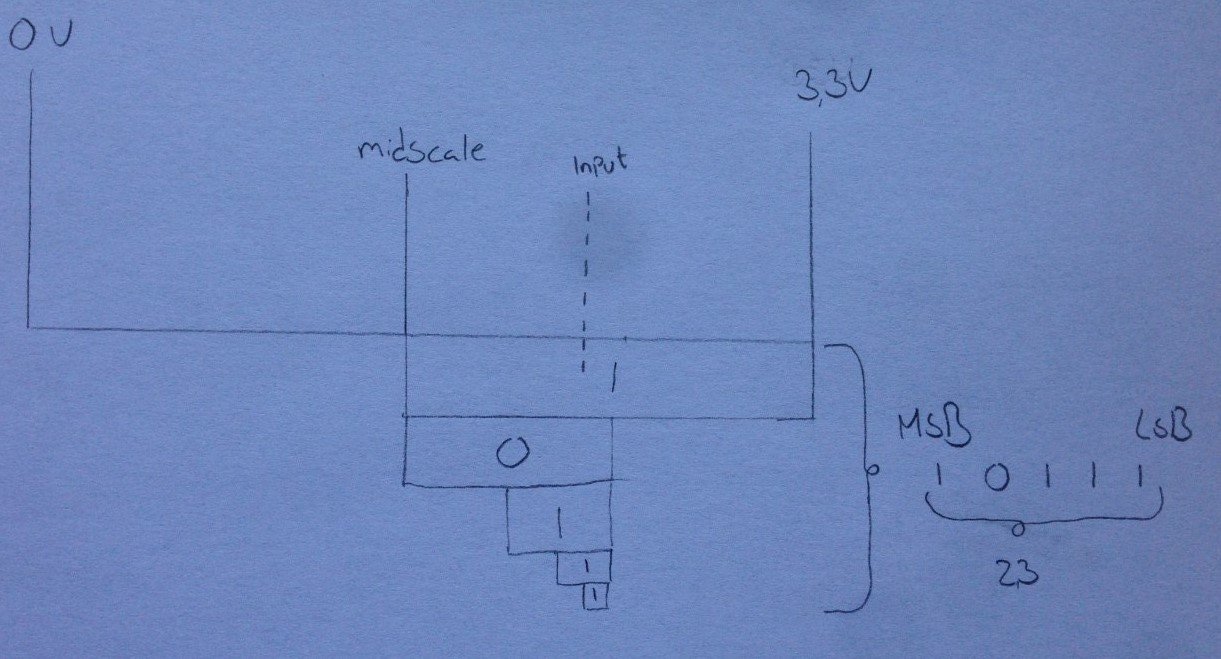
\includegraphics[width=\textwidth]{Afsnit/DesignOgImplementering/images/ADC}
	\caption{ADC opbygning}
	\label{fig:pot}
	\end{figure}

Der er blevet målt med en vinkel måler for at over holde kravene i kravspecifikationen\textbf{\#ref Reference til kravspecikation (ikke funktionelle krav)}. Hvor der blev fundet frem til en min og max hvor motoren må køre i mellem. \\
\\
Min=915 mV\\
\\
Max = 2000mV\\
\\
Disse værdier er aflæst fra PSoC’en, da den har en ref spændingen på 3.3V vil den have lavere værdier end hvad der bliver sendt ud fra Potentiometeret.


\begin{equation}
 \frac {5V} {3.3V}= 1.515
\end{equation}
Der er en forskel på ca. 1.515   mellem potentiometer og ADC. Så ADC er ca. 1,515 mindre end hvad potentiometer sender ud.
\\
For at forstå hvordan ADC’en og potentiometeret fungerer henvises der til dokumentatioen.

\subsection{Affyringsmekanisme}
Affyringsmekanismen er bygget op af en motor; et motorstyringskredsløb; et detektorkredsløb, der skal detektere, at motoren kun kører en enkelt omgang, når der skydes; og en kanon, som er bygget op af noget mekanik og LEGO. 

\subsubsection{Detektor}
Detektorens formål er at detektere, hvornår motoren er kørt en omgang, og derefter slukke den. 

\subsubsection{Motorstyring}


\subsubsection{Kanon}
Selve kanonen i systemet er bygget op af to træplader og LEGO. Den ene træplade skal kunne dreje fra side til side, således at det er muligt at sigte i den horisontale retning. Den vertikale retning er bygget af LEGO, ligesom selve kanonen også er bygget i LEGO. 

\section{Software}

\subsection{SPI - Devkit8000}
Candydriveren sørger for SPI-kommunikationen fra Devkit8000 til PSoC0. Driveren er skrevet i c, hvilket er typisk for drivere til linuxplatforme.\\
SPI-kommunikationen er implementeret med SPI bus nummer 1, SPI chip-select 0 og en hastighed på 1 MHz (et godt stykke under max på 20 MHz for en sikkerhedsskyld). Desuden starter clocken højt og data ændres på falling edge og aflæses på rising edge. Dermed bliver SPI Clock Mode 3. Derudover sendes der 8 bit pr transmission, hvilket passer med SPI-protokollen for projektet.\\
For at kunne anvende driveren, når SPI er tilsluttet, er der oprettet et hotplugmodul, som fortæller kernen, at der er et SPI device, som matcher driveren. Det kan SPI-forbindelsen ikke selv gøre, som usb fx kan. Selve driveren er i candygun.c opbygget som en char driver. For at holde forskellige funktionaliteter adskilt er alle funktioner, der har med SPI at gøre, implementeret i filen candygun-spi-c. Så når der fx skal requestes en SPI ressource i init-funktionen i candygun.c, så anvender driveren en funktion fra candygun-spi.c til det. I probe-funktionen sættes bits\textunderscore per\textunderscore word til 8, da vi sender otte bit som nævnt tidligere. I exit-funktionen anvender candygun.c igen en funktion fra candygun-spi.c - denne gang til at frigive SPI ressourcen. I write-metoden gives der data med fra brugeren. I dette tilfælde udgøres brugeren af Interface driveren og dataet er en 8 bit kommando fra SPI-protokollen. Dog er dataet fra brugeren i første omgang læst ind som en charstreng. I write-metoden bliver det så lavet om til en int.  For at overføre dataet på en sikker måde anvendes funktionen copy\textunderscore from\textunderscore user() til at overføre data fra brugeren. Write-funktionen fra candygun.c anvender derefter en write-funktion fra candygun-spi.c, hvor den sender brugerinputtet med. I den spi-relaterede write-funktion bliver bruger inputtet lagt i transfer bufferen og der NULL bliver lagt i receive bufferen, og med spi\textunderscore sync-funktionen bliver det sendt.\\ 
Ofte ville der en spi read-funktion først indeholde en write-del, som fortalte SPI-slaven, hvad der skulle læses over i bufferen. Det ville typisk efterfølges af et delay og så en read-del. Men i dette projekt skal der ofte afventes et brugerinput, som ikke kan styres af et fast delay, og der skal generelt sendes en aktiv kommando før der læses. Derfor er det besluttet at read-funktionen kun indeholder en read-del i transmissionen. Dermed skal write-funktionen altid aktivt anvendes inden der læses, da PSoC0 ellers ikke ved, hvad der skal gøres/lægges i bufferen.\\
Når funktionen har modtaget resultatet fra transmissionen returneres det til brugeren med funktionen copy\textunderscore to\textunderscore user(), som igen sørger for at overførslen af data foregår på en sikker måde.   


\subsection{Interface Driver}
Interface driveren fungerer som bindeled mellem brugergrænsefladen og candydriveren på Devkit8000. Den indeholder tre funktioner. Funktionerne anvendes i use case 2 til at teste kommunikationsforbindelserne i resten af systemet. Interface driveren er designet og implementeret i C++ og gør brug af klasserelationen arv. Et klassediagram for interface driveren se på figur  \ref{fig:idriveruc2}.\\

\begin{figure}[H]
	\centering
	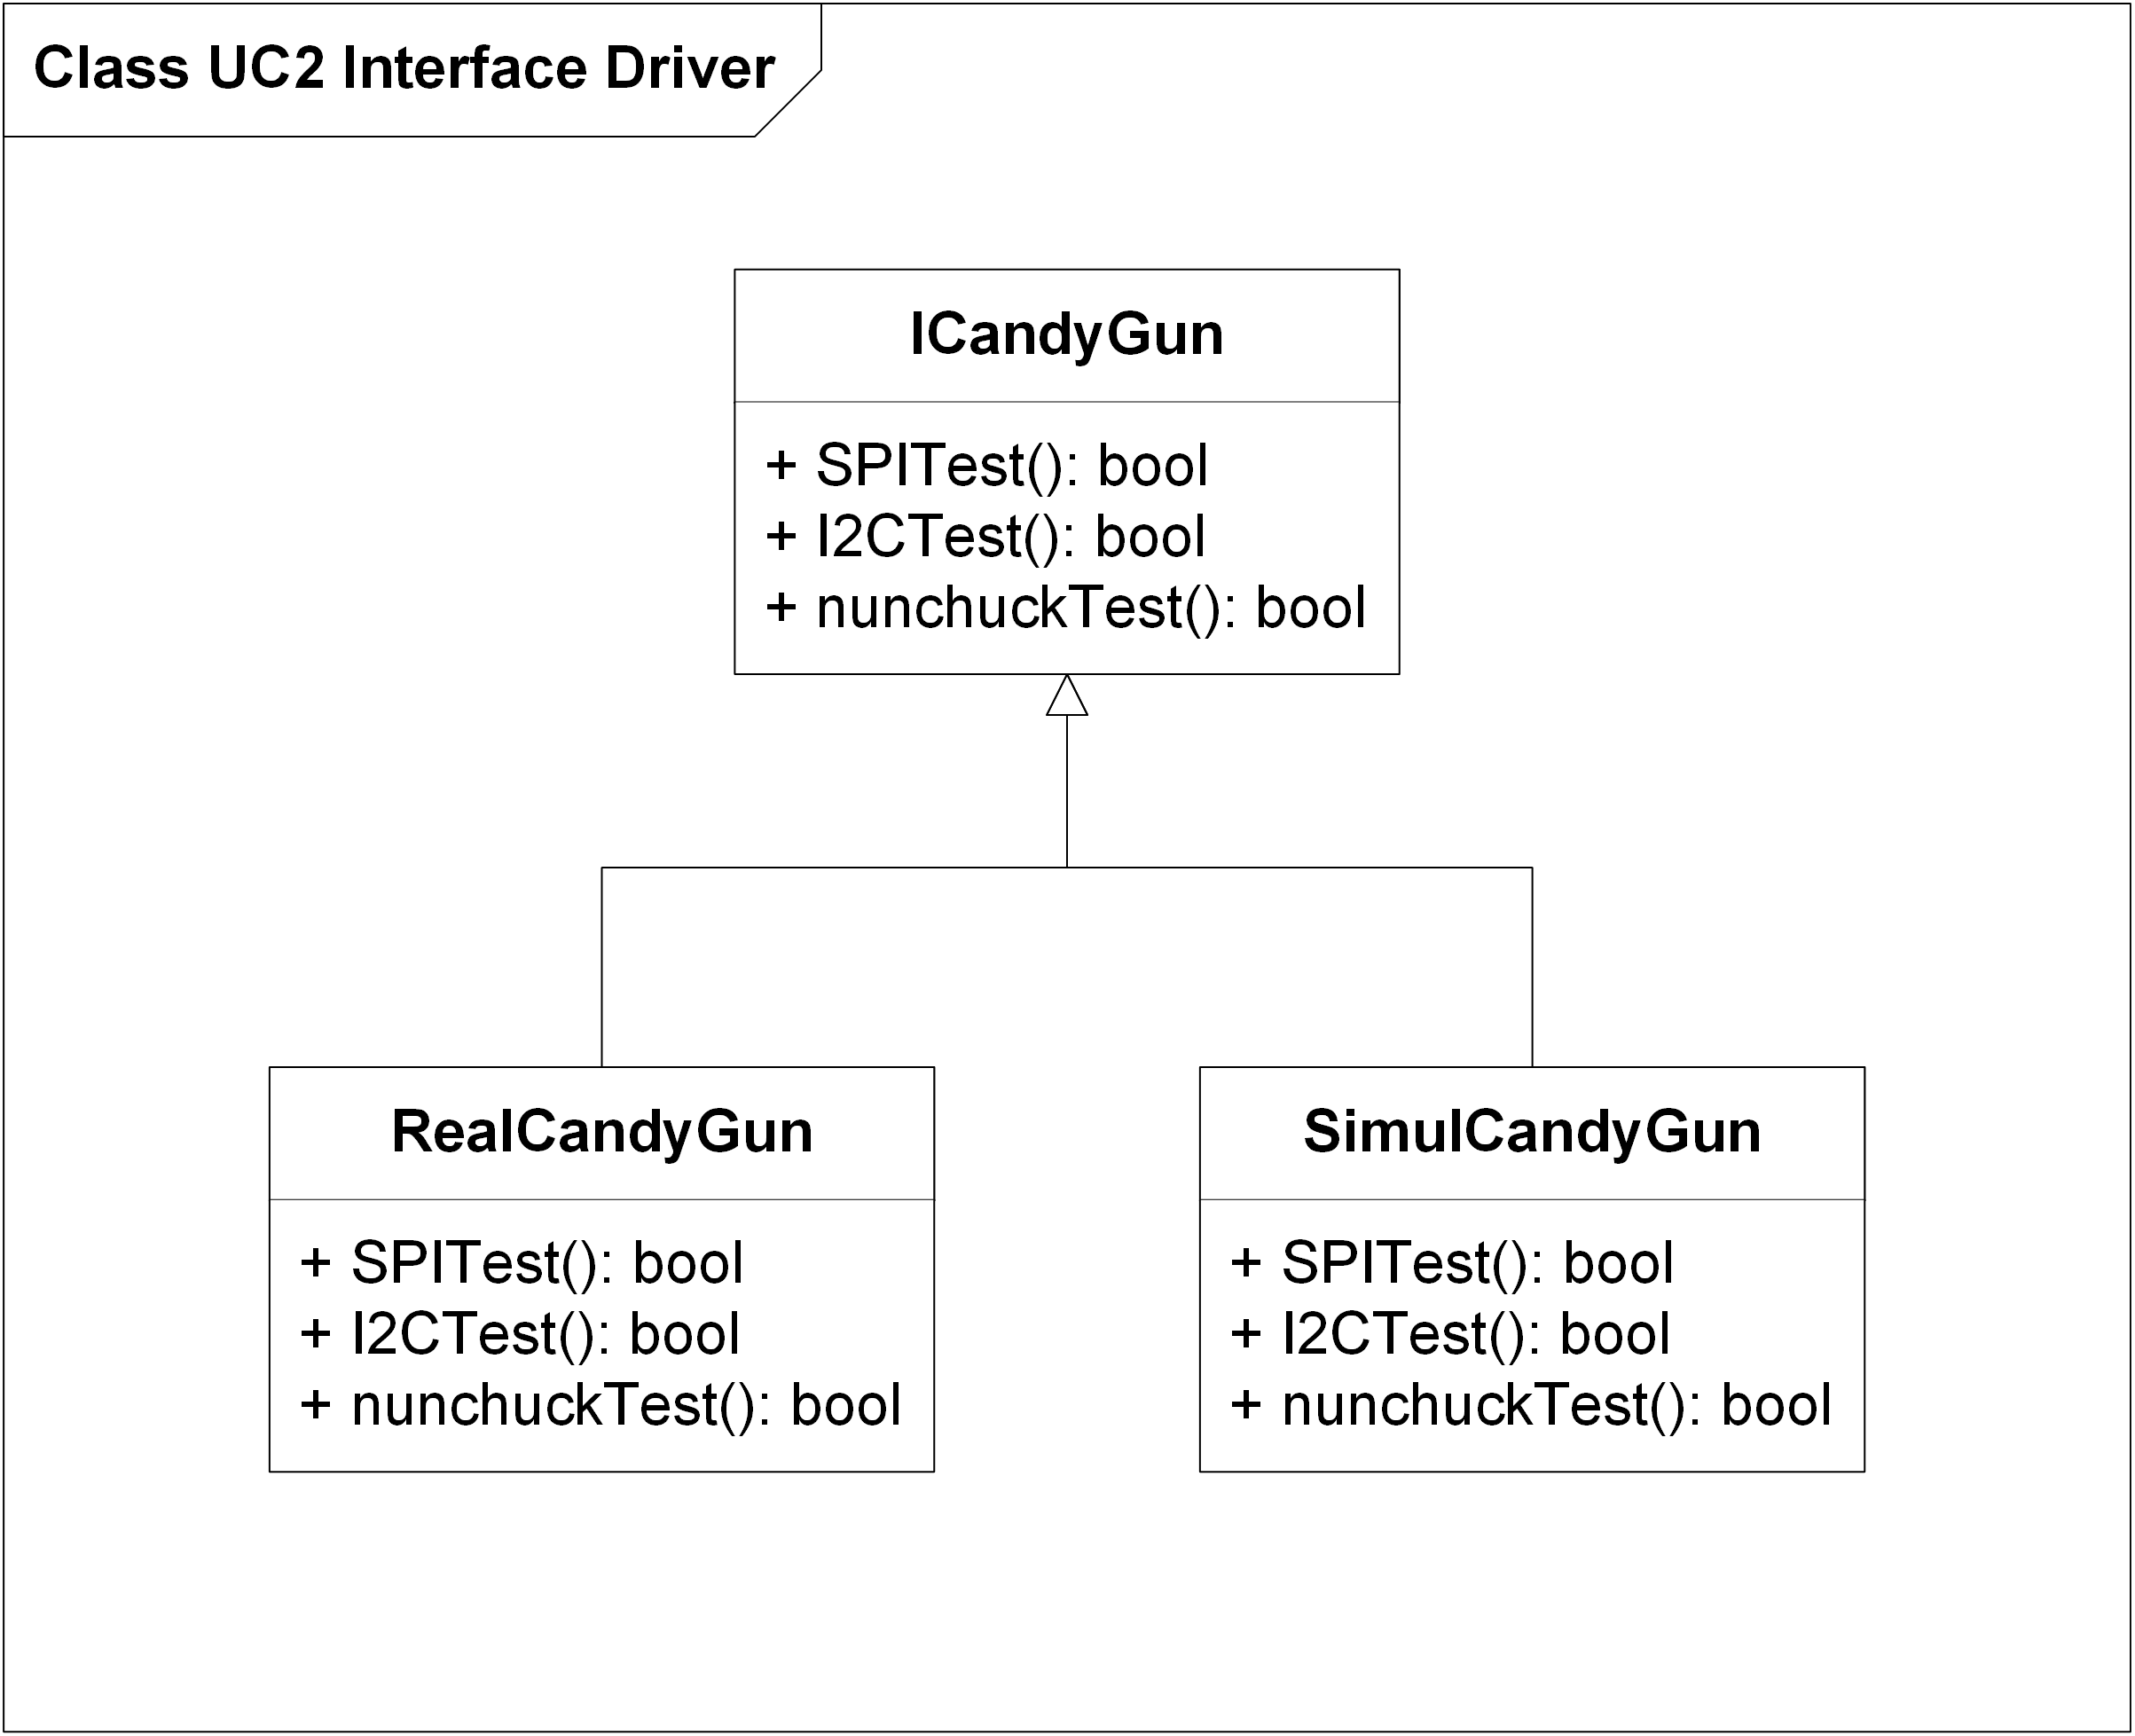
\includegraphics[width=\textwidth]{Afsnit/DesignOgImplementering/images/IdriverKlasseDiagram}
	\caption{Interface driver for UC2}
	\label{fig:idriveruc2}
\end{figure}

Basisklassen er ICandyGun. Det er en abstrakt klasse, da den udelukkende indeholder virtuelle metoder. Derudover er der to afledte klasser; SimulCandyGun og RealCandyGun. SimulCandyGun implementerer metoderne til at simulere respons fra Candydriveren. Dermed kan brugergrænsefladen testes uafhængigt af de resterende dele af systemet. Simuleringen er implementeret med \textit{srand()}-funktionen fra \textit{cstdlib}-biblioteket, som returnerer et tilfældigt tal, som her bliver mellem 0 og 1. I RealCandyGun-klassen er metoderne implementeret efter den reelle SPI-protokol og med de nødvendige funktioner til at skrive til et kernemodul. Fx open(), close(), read () og write(). Da interface driveren er implementeret med arv, skal der ikke foretages betydelige ændringer i brugergrænsefladen, når der skiftes mellem simuleringsklassen og den rigtige version. Dermed opnås lav kobling. \\
De tre funktioner som Interface driveren indeholder i forbindelse med use case 2 (test use casen) er: SPITest(), I2CTest(), NunchuckTest(). Hver af de tre funktioner anvendes til at starte en test af de forskellige kommunikationsforbindelser: SPI, I2C og brugerinputet fra nunchucken. Alle funktionerne returnerer en bool, som enten er true eller false, alt efter om testen var succesful eller ej. Når der skal startes en test, åbner den pågældende funktion filen \textit{dev/candygun} og skriver SPI-kommandoen for \textit{start test} til filen. Derefter venter funktionen ét sekund og læser så svaret fra filen. Da der i nunchucktesten ventes på et brugerinput, og brugeren skal have lidt tid til at trykke på nunchuck-knappen, er der oprettet en while-løkke, som tjekker flere gange om testen returnerer true. Hvis testen ikke returnerer true ved første check, venter funktionen atter et sekund og tjekker igen. Det gør den op til 15 gange og melder derefter om fejl, hvis ikke den returnerer true inden.\\
Brugergrænsefladen anvender interface driveren ved at inkludere headerfilerne og oprette en ICandyGun pointer, der peger på en instans af én af de to afledte klasser. Ved at pakke kommunikationen  til kernemodulet for candydriveren væk i funktioner kan brugergrænsefladen anvende funktionerne uden at kende til SPI-protokollen. Det sikrer igen lav kobling, og i tilfælde hvor det kunne ønskes, at SPI-kommunikationen kan erstattes af en anden kommunikationsform, kan det gøres uden, at der skal foretages ændringer i brugergrænsefladen.\\
 
\subsection{Brugergrænseflade}
\begin{figure}[H]
	\centering
	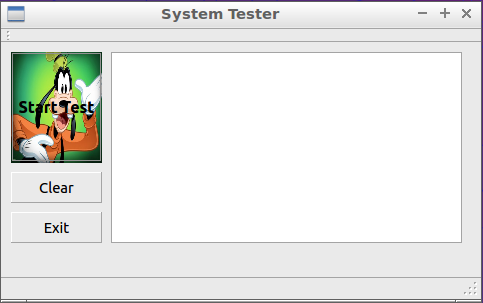
\includegraphics[width=\textwidth]{Afsnit/DesignOgImplementering/images/GUIPic}
	\caption{Brugergrænseflade for usecase 2}
	\label{fig:GUIPic}
\end{figure}

Brugergrænsefladen er lavet med det indbyggede design framework i QT Creator 5.
QT frameworket opretter "hovedvinduet" i brugergrænsefladen som en klasse. Knapperne tilføjes som private slots i klassen
hvilket gør dem i stand til interagere i brugergrænsefladen. Når en knap er assignet til et slot i klassen, og der trykkes på den pågældende knap, bliver det assignede signal broadcastet
og slot-funktionen bliver kørt. Alle tre knapper i brugergrænsefladen er assignet signal-typen "clicked()". Signalet broadcastets når knappen trykkes.

\begin{figure}[H]
	\centering
	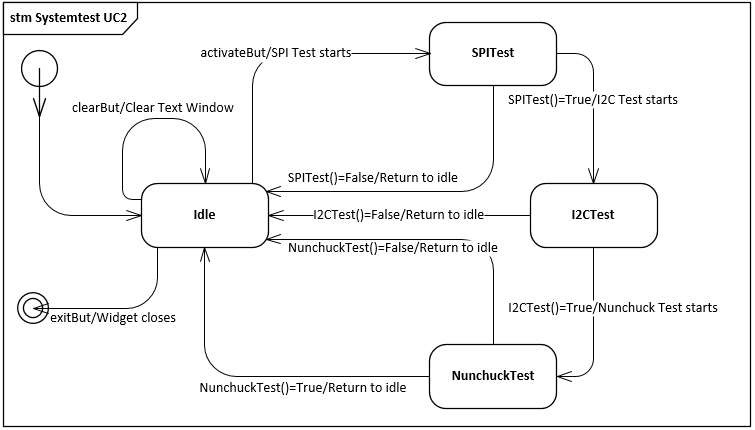
\includegraphics[width=1.2\textwidth]{Afsnit/DesignOgImplementering/images/StateMachineUC2}
	\caption{State machine for brugergrænsefladen for usecase 2}
	\label{fig:StateMachineUC2}
\end{figure}

Brugergrænsefladen for UC2 er en simpel test-konsol. Den består af 3 knapper og et tekstvindue. Brugergrænsefladen interfacer med SPI-protokollen, gennem vores interface driver. Den første knap, Start test, initierer UC2. Efterhånden som testen løbes igennem kaldes test funktionerne, og ved hjælp af if-conditions, bliver der tjekket på retur-værdierne fra interface-funktionerne. Hvis retur-værdien er true, skrives der en "--test successful" besked i tekstvinduet. og widgeten kører videre. Hvis retur-værdien er false, skrives der en "--test unsuccessful" i tekstvinduet og widgeten returnerer til idle tilstand. Når alle test er successful, skrives "System test successful, system is ready for use" til tekstvinduet, og widgeten returnerer til idle tilstand. Den anden knap, Clear, clearer tekstvinduet til blank tilstand. Den tredje knap, Exit, lukker widgeten.

\subsection{Nunchuck}
Til styring af kanonen bruges en Wii-nunchuck. Følgende afsnit beskriver PSoC0's håndtering af data fra Wii-nunchuck.

\subsubsection{Afkodning af Wii-Nunchuck Data Bytes}
Aflæste bytes fra Wii-Nunchuck - indeholdende tilstanden af knapperne og det analoge stick - er kodet når de oprindeligt modtages via I2C bussen. Disse bytes skal altså afkodes før deres værdier er brugbare. Afkodningen af hver byte sker ved brug af følgende formel:

\textit{AfkodetByte = (AflæstByte XOR 0x17) + 0x17}

Fra formlen kan det ses at den aflæste byte skal \textit{XOR}'s (Exclusive Or) med værdien 0x17, hvorefter dette resultat skal adderes med værdien 0x17.

\subsubsection{Kalibrering af Wii-Nunchuck Analog Stick}
De afkodede bytes for Wii-Nunchuck's analoge stick har definerede standardværdier for dets forskellige fysiske positioner. Disse værdier findes i tabel \ref{tabel:WiiNunchuckStickPositioner}

\begin{table}[H]
	\centering
	\begin{tabular}{|l|l|}
		\hline
		X-akse helt til venstre & 0x1E \\ \hline
		X-akse helt til højre   & 0xE1 \\ \hline
		X-akse centreret        & 0x7E \\ \hline
		Y-akse centreret        & 0x7B \\ \hline
		Y-akse helt frem        & 0x1D \\ \hline
		Y-akse helt tilbage     & 0xDF \\ \hline
	\end{tabular}
	\caption{Standardværdier for fysiske positioner af Wii-Nunchuck's analoge stick}
	\label{tabel:WiiNunchuckStickPositioner}
\end{table}

I praksis skal de afkodede værdier for det analoge stick kalibreres, da slør pga. brug gør at de ideale værdier ikke rammes. 

I projektet er de afkodede værdier for det analoge stick kalibreret med værdien -15 (0x0F i hexadecimal), altså ser den endelige formel for afkodning samt kalibrering således ud:

\textit{AfkodetByte = (AflæstByte XOR 0x17) + 0x17 - 0x0F}

\subsection{PSoC Software}
De følgende klassediagrammer på figur \ref{figure:klassediagramPSoC0} og \ref{figure:klassediagramPSoC1} giver et overblik over hvilke klasser der bliver gjort brug af på PSoC0 og PSoC1. De efterfølgende afsnit vil beskrive klasserne og deres funktioner.

\begin{figure}[H]
	\centering
	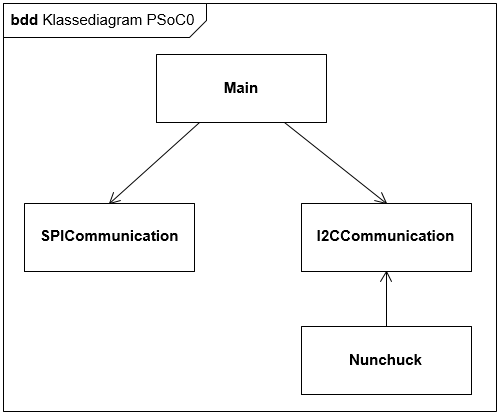
\includegraphics[width=.7\textwidth]{DesignOgImplementering/images/PSoC0KlassediagramOversigt}
	\caption{Klassediagram oversigt for PSoC0}
	\label{figure:klassediagramPSoC0}
\end{figure}

\begin{figure}[H]
	\centering
	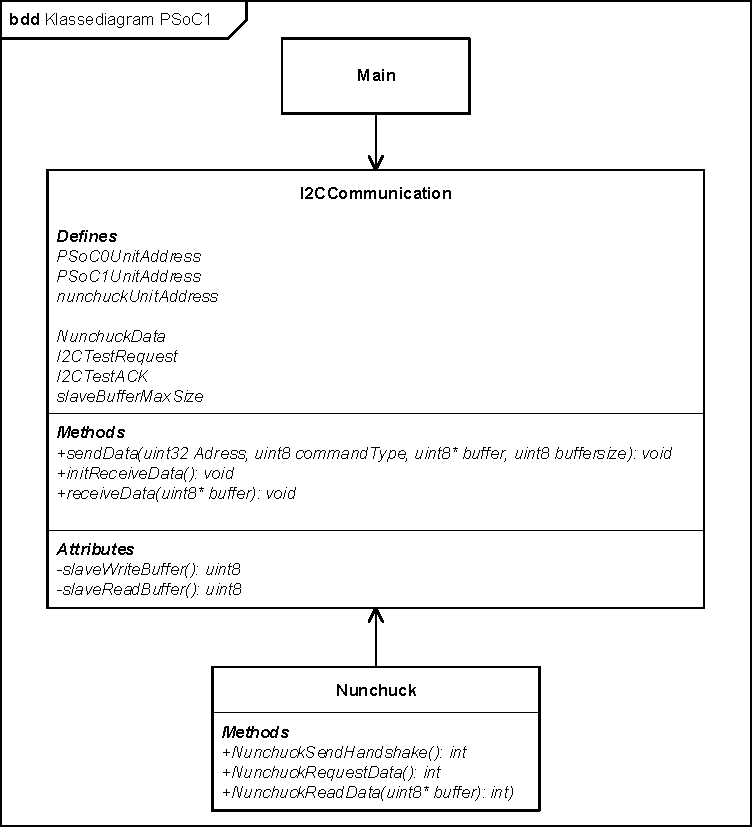
\includegraphics[width=.7\textwidth]{DesignOgImplementering/images/PSoC1KlassediagramOversigt}
	\caption{Klassediagram oversigt for PSoC1}
	\label{figure:klassediagramPSoC1}
\end{figure}

\subsection{I2CCommunication}
I dette afsnit vil softwaren der omhandler I2C-kommunikation blive beskrevet. Dette inkluderer et klassediagram, samt en klassebeskrivelse.
\subsubsection{Klassediagram}
På figur \ref{figure:klassediagramI2CCommunication} ses klassediagrammet for I2CCommunication. 
\begin{figure}[H]
	\centering
	%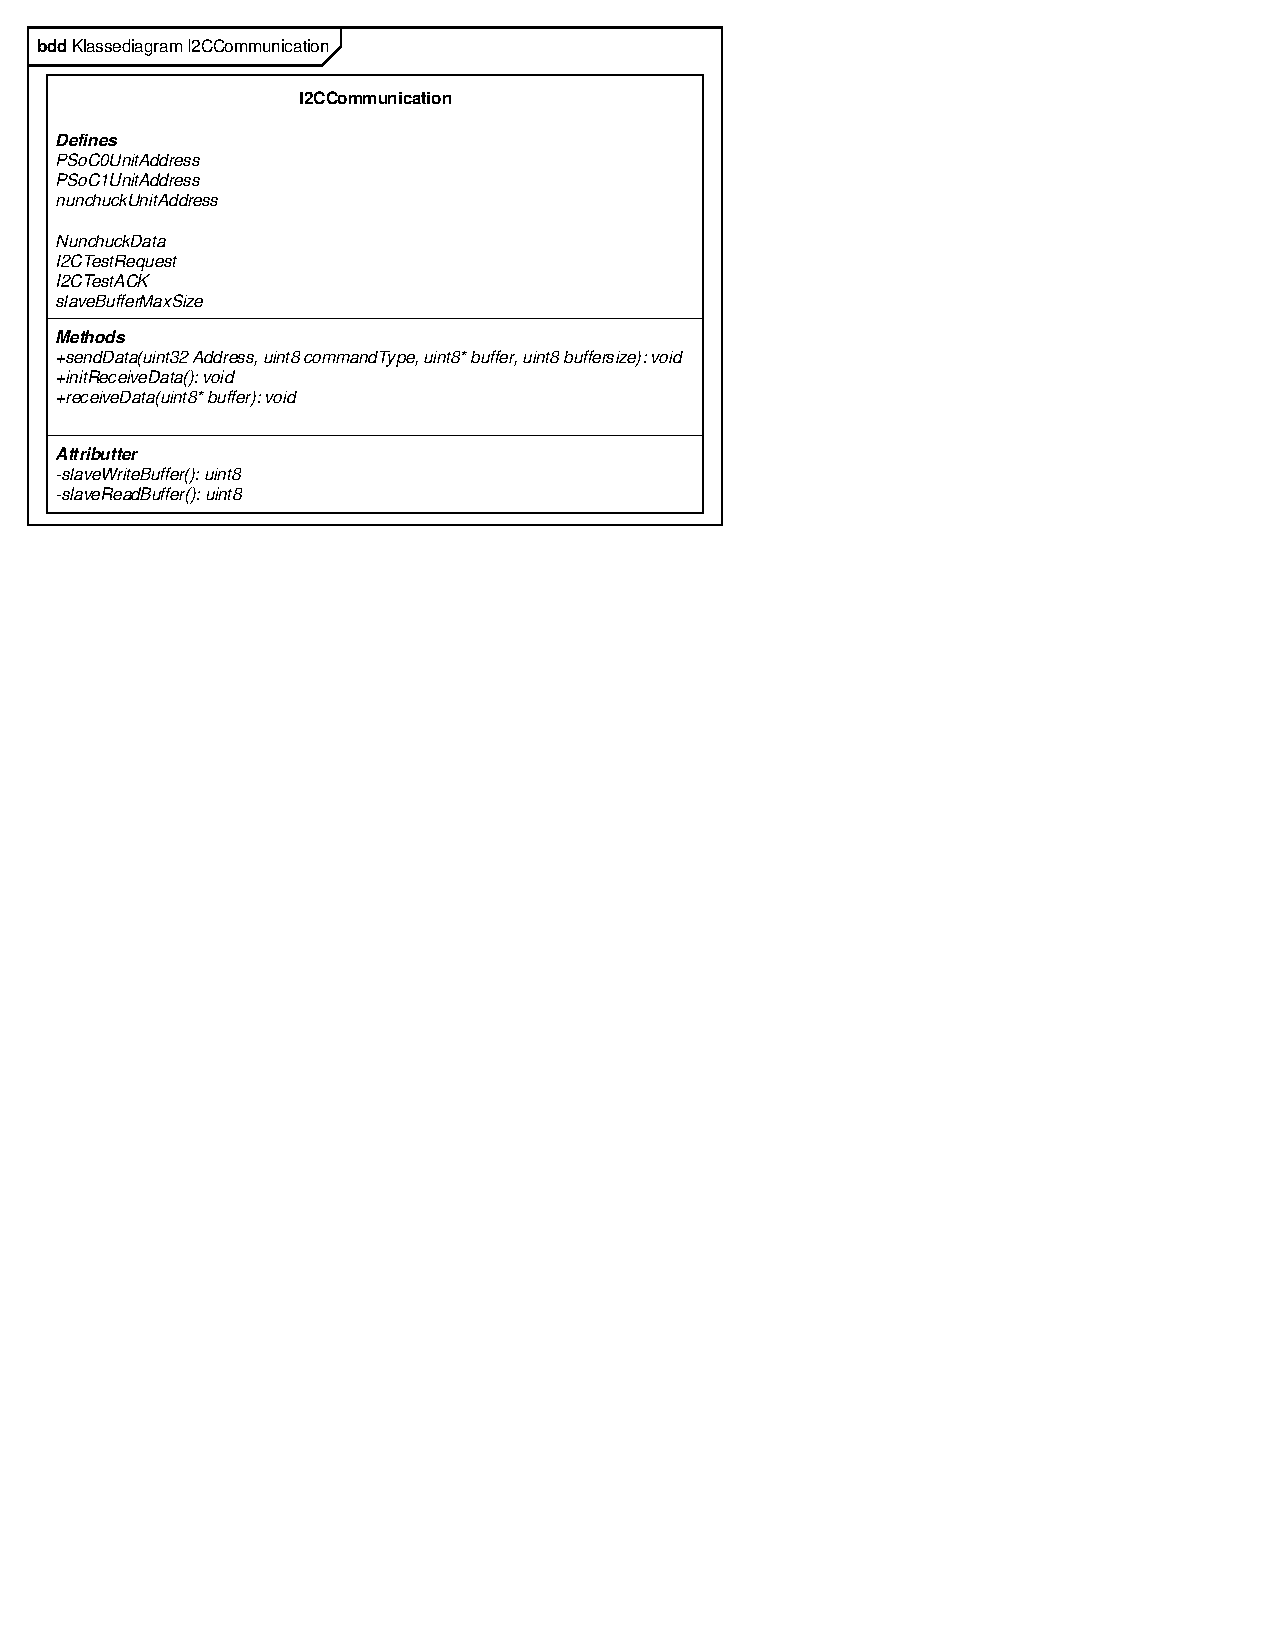
\includegraphics[width=0.9\textwidth, trim={0 19cm 9cm 0},clip]{DesignOgImplementering/images/I2CCommunication.pdf}
	\includegraphics[]{DesignOgImplementering/images/I2CCommunication}
	%\includegraphics[width =0.9\textwidth]{DesignOgImplementering/images/I2CCommunication2}
	\caption{Klassediagram for I2CCommunication klassen}
	\label{figure:klassediagramI2CCommunication}
\end{figure}

\subsection{Nunchuck}
I dette afsnit vil softwaren der specifikt omhandler kommunikationen mellem PSoC0 og Nunchucken blive beskrevet. Dette gøres vha. et klassediagram og klassebeskrivelser.

\subsubsection{Klassediagram}
På figur \ref{figure:NunchuckKlassediagram} ses klassediagrammet for Nunchuck klassen.

\begin{figure}[H]
	\centering
	\includegraphics[]{DesignOgImplementering/images/nunchuck}
	\caption{Klassediagram for klassen Nunchuck}
	\label{figure:NunchuckKlassediagram}
\end{figure}

\subsection{SPI - PSoC}
I dette afsnit vil softwaren der specifikt omhandler SPI-kommunikationen mellem PSoC0 og DevKit8000 blive beskrevet. Dette gøres vha. et klassediagram og klassebeskrivelser

\subsubsection{Klassediagram}
På figur \ref{figure:KlassediagramSPICommunication} ses klassediagrammet over SPICommunication klassen.

\begin{figure}[H]
	\centering
	\includegraphics[]{DesignOgImplementering/images/SPICommunication}
	\caption{Klassediagram over klassen SPICommunication}
	\label{figure:KlassediagramSPICommunication}
\end{figure}
	\chapter{Modultest}

\section{Software}

\subsection{Modultest af Wii-Nunchuck}
På PSoC0 er der software til aflæsning af Wii-Nunchuck input data. Følgende afsnit beskriver test af dette software.

Aflæsning af Wii-Nunchuck sker i to skridt, som begge verificeres ved modul test. Først skal der sendes et \textit{Handshake} fra PSoC0 til Wii-Nunchuck for at initialisere data udveksling, og herefter sker data udveksling hver gang PSoC0 sender en anmodning om det. Disse to skridt modultestes her.

\textbf{Test af Wii-Nunchuck Handshake}

\textbf{Test af data udveksling mellem PSoC0 og Wii-Nunchuck} 

PSoC0 blev programmeret til kontinuert aflæsning af Wii-Nunchuck. For at verificere data udveksling mellem PSoC0 og Wii-Nunchuck blev I2C bussen målt ved brug af Logic Analyzer fra Analog Discovery.

Data udveksling sker i to skridt. Først sender PSoC0 en byte med værdien 0 (0x00 i hexadecimal). Herefter sker den faktiske aflæsning, PSoC0 aflæser Wii-Nunchuck. Begge skridt testes her.

\textbf{Afsendelse af 0x00 byte}

Den første forventede I2C besked er en \textit{0x00} byte fra PSoC0 for at starte en ny aflæsning. På figur \ref{fig:NunchuckWriteValues} ses aflæsningen af I2C bussen på tidspunktet hvor anmodningen til Wii-Nunchuck bliver udført. Dette er en tidslinje læst fra ventre til højre.

\begin{figure}[H]
	\centering
	\includegraphics[width=\textwidth]{Test/images/writerequest}
	\caption{}
	\label{fig:NunchuckWriteValues}
\end{figure}

Det kan på figur \ref{fig:NunchuckWriteValues} ses at den første besked der måles er af typen "WR" (Write) til addressen 0x52 (Wii-Nunchuck I2C Slave Addressen). Hertil kommer et tilhørende \textit{ACK} (Acknowledge) fra Wii-Nunchuck. Til sidst sendes dataen Ox00 efterfulgt af at ACK fra Wii-Nunchuck. Til sidst afsluttes I2C transaktionen ved "Stop".

Det kan altså konkluderes at målingen er i overensstemmelse med forventningen om at en 0x00 byte skal sendes til Wii-Nunchuck for opstart af dataudveksling.

\textbf{Aflæsning af Wii-Nunchuck}

Efter vellykket afsendelse af 0x00 byten sker den egentlige aflæsning af Wii-Nunchuk input dataen.

Her forventes en række beskeder indeholdende 

På figur \ref{fig:NunchuckReadValues} ses I2C beskederne der bliver udvekslet mellem PSoC0 og Wii-Nunchuck efter vellykket Wii-Nunchuck Handshake. 

\begin{figure}[H]
	\centering
	\includegraphics[width=\textwidth]{Test/images/readvaluesEdited.png}
	\caption{Tidslinje af aflæste I2C beskeder af PSoC0 fra Wii-Nunchuck}
	\label{fig:NunchuckReadValues}
\end{figure}

\subsection{SPI Protokol}
Devkittet kommunikerer over en SPI bus. Kommunikationen følger SPI kommunikations protokollen, som er beskrevet i afsnit \ref{afsnit:spiprotokol}. Dette afsnit beskriver test af denne protokol.

\subsubsection{SPI Bus Test}
Test af SPI bussen udføres i to dele. Første del af testen udføres ved at sende kommandotypen for start af SPI test i terminalen, og derefter verificere den sendte data vha. Analog Discovery. Den anden del af testen, er at aflæse returbeskeden på bussen med Analog Discovery. Målet med denne test, er at læse kommandotypen "SPI\_OK", der indikerer en successful aflæsning af SPI-slaven.  På figur \ref{figure:SpiTestSetup} ses test opsætningen. Devkit8000, PSoC0s SPI-bus og Analog Discovery  er forbundet til hinanden igennem fumlebrættet. PSoC0 og PSoC1's I2C-forbindelser forbindes til nunchucken igennem fumlebrættet, adskilt fra SPI-forbindelserne.


\begin{figure}[H]
	\centering
	\includegraphics[width=\textwidth]{Test/images/SPItest/SpiTestSetup}
	\caption{Opsætning for SPI-test}
	\label{figure:SpiTestSetup}
\end{figure}


I testen afsendes SPI test kommandotypen, som har værdien 0xF1 jf. tabel \ref{tabel:spiKommandoType}. For at verificere, at kommandotypen er sendt ud på SPI-bussen korrekt, blev Analog Discovery's 'Logic Analyzer' brugt til at aflæse SPI-bussen. Det var forventet at 0xF1 blev aflæst på bussen. Det afmålte resultat stemte overens med det forventede. Målingen ses på figur \ref{fig:SPItestkommandotype}. 

\begin{figure}[H]
	\centering
	\includegraphics[width=\textwidth]{Test/images/SPItest/SPItestkommandotype}
	\caption{Måling af kommandotype for start SPI test}
	\label{fig:SPItestkommandotype}
\end{figure}

Hvis SPI-kommunikationen fungerer korrekt, er det forventet at der aflæses 0xD1 på SPI-bussen, da dette betyder 'SPI\_OK' jf. tabel \ref{tabel:spiKommandoType}. Måling af returbeskeden ses på figur \ref{fig:SPItestSPIOK}.

\begin{figure}[H]
	\centering
	\includegraphics[width=\textwidth]{Test/images/SPItest/SPItestSPIOK1}
	\caption{Måling af returbesked for start SPI test} 
	\label{fig:SPItestSPIOK}
\end{figure}

På figur \ref{fig:SPItestSPIOK} ses at returbeskeden har den forventede værdi 0xD1, som indikerer at SPI bus testens første del er gennemført uden fejl.

Ud fra testenes resultater kan det konkluderes at implementeringen af SPI protokollen fungerer efter hensigten.



\subsection{I2C Protokol}
PSoC0 og PSoC1 kommunikerer over en I2C bus via I2C protokollen beskrevet i afsnit \ref{afsnit:I2CProtokol}. Dette afsnit beskriver test af denne protokol. Følgende test tager udgangspunkt i kommandotypen \textit{NunchuckData} beskrevet i tabel \ref{table:I2CKommandoer}).

\subsubsection{Test af NunchuckData kommandotype} 

Testen blev udført i to dele. I første del måles I2C bussen ved brug af Analog Discovery's Logic Analyzer; for at verificere at den forventede kommandotype bliver overført via bussen. Anden del verificerer at den overførte data er modtaget korrekt via PSoC Creator's debugger.

\subsubsection{NunchuckData kommandotype test del 1}

I testen afsendes, som nævnt i afsnittets indledning, kommandotypen NunchuckData. Som vist i tabel \ref{table:I2CKommandoer} har denne kommandotype ID'et 0xA2, hvor de efterfølgende 3 data bytes indeholder input dataen fra Wii-Nunchuck.

Det forventede resultat af målingen er at første byte er kommandoentypens ID, som har værdien 0x2A. Kommandoens data - de efterfølgende bytes - verificeres først i anden del, disse indgår altså ikke i følgende måling. 

Målingen ses på figur \ref{fig:NunchuckDataCommand}.

\begin{figure}[H]
	\centering
	\includegraphics[width=1.2\textwidth]{Test/images/ShowsNunchuckDataCommand.png}
	\caption{Tidslinje af målt I2C kommandotype}
	\label{fig:NunchuckDataCommand}
\end{figure}

Det kan ses på figur \ref{fig:NunchuckDataCommand} at I2C overførslen starter med en I2C \textit{write}, som får et successfuldt acknowledge fra slaven PSoC1. Herefter kan det ses at den næste byte der sendes har værdien 0x2A. Denne byte er kommandoentypens ID, og er altså som forventet 0x2A.

Det kan altså verificeres at kommandoen overføres via I2C bussen. Dataens integritet er dog ikke inkluderet i denne del, og testes i del 2.

\subsubsection{NunchuckData kommandotype test del 2}
For at verificere integriteten af den data der sendes mellem PSoC0 og PSoC1, bruges PSoC Creators indbyggede debugger. Igen er det kommandotypen NunchuckData der sendes mellem de to enheder, hvor de medfølgende data bytes fortolkes.

Testen gennemføres ved at fortolke den modtagne data tre gange, hvor nunchucken er i forskellige tilstande (hvilken retning det analoge stik er trykket) i hver test. Værdierne sammenlignes de forventede standardværdier som ses i tabellen på side 3 i \cite[I2C Interface with Wii Nunchuck]{nunchuck}. Da testene kun er fokuserede på, hvilken retning den analoge stick er presset, er det altså kun receivedDataBuffer[1] (den analoge stick x-akse) og receivedDataBuffer[2] (den analoge pinds y-akse) der er relevante for testen. Når den analoge stick er presset til venstre, forventes det ifølge tabel \ref{tabel:WiiNunchuckStickPositioner} at receivedDataBuffer[1] er lig 0x1E og receivedDataBuffer[2] er 0x7B. Når den analoge stick er presset op, forventes det at receivedDataBuffer[1] er 0x7E og receivedDataBuffer[2] er 0xDF. Når der ikke er noget input på Nunchucken forventes det at receivedDataBuffer[1] er 0x7E og receivedDataBuffer[2] er 0x7B. Målingerne for testene kan ses på figur \ref{fig:I2CProtocolReadNoInput}, \ref{fig:I2CProtocolReadLeftAnalog} og \ref{fig:I2CProtocolReadUpAnalog}.

\begin{figure}[H]
	\centering
	\includegraphics[width=.5\textwidth]{Test/images/I2CProtocolReadNoInput.png}
	\caption{Afmåling af modtager-buffer på PSoC1 efter at have modtaget "NunchuckData" kommando typen. Intet input på Nunchuck'en}
	\label{fig:I2CProtocolReadNoInput}
\end{figure}

\begin{figure}[H]
	\centering
	\includegraphics[width=.5\textwidth]{Test/images/I2CProtocolReadLeftAnalog.png}
	\caption{Afmåling af modtager-buffer på PSoC1 efter at have modtaget "NunchuckData" kommando typen. Den analoge stick er presset til venstre på Nunchuck'en}
	\label{fig:I2CProtocolReadLeftAnalog}
\end{figure}

\begin{figure}[H]
	\centering
	\includegraphics[width=.5\textwidth]{Test/images/I2CProtocolReadUpAnalog.png}
	\caption{Afmåling af modtager-buffer på PSoC1 efter at have modtaget "NunchuckData" kommando typen. Den analoge stick er presset frem på Nunchuck'en}
	\label{fig:I2CProtocolReadUpAnalog}
\end{figure}

På figur \ref{fig:I2CProtocolReadLeftAnalog} ses afmålingen af modtager-bufferen når Nunchuckens analoge stick er presset helt til venstre. ReceivedDataBuffer[1] blev aflæst til 0x1E og receivedDataBuffer[2] blev aflæst til 0x7C. ReceivedDataBuffer[1] stemmer overens med forventningerne. ReceivedDataBuffer[2] har en lille afvigelse (oversat til decimaltal blev der målt 124, hvor der forventes 123). Denne afvigelse kan skyldes, at det analoge stick ikke blev presset direkte til venstre, men at den også er blevet presset en smule frem under målingen.

På figur \ref{fig:I2CProtocolReadUpAnalog} ses afmålingen af modtager-bufferen når Nunchuckens analoge stick er presset frem. ReceivedDataBuffer[1] blev aflæst til 0x82, hvor det var forventet 0x7E. Dette er en afvigelse fra de forventede resultater med 4, og kan skyldes at det analoge stick ikke var helt centreret idét den blev presset frem under målingen. ReceivedDataBuffer[2] blev aflæst til 0xDF, hvilket stemmer overens med de forventede målinger.

På figur \ref{fig:I2CProtocolReadNoInput} ses afmålingen af modtager-bufferen når der ikke er noget brugerinput på nunchuckens analoge stick. ReceivedDataBuffer[1] blev aflæst til 0x7F, hvor det forventede resultat var 0x7E. Denne afvigelse kan skyldes at det analoge stick ikke stod helt i midten under målingen (Det analoge stick er lidt "løs" og kan defor godt finde hvile i en position der ikke er fuldt centreret). ReceivedDataBuffer[2] blev aflæst til 0x7D, hvor det forventede resultat var 0x7B. Igen kan denne afvigelse skyldes at det analoge stick ikke var i centrum under målingen.

Ud fra testen kan det konkluderes at implementeringen af I2C-protokollen fungerer efter hensigten.

\section{Hardware}
\subsection{H-bro} 

\textbf{Formål}
\\ Formålet med denne test er at viser at motor kan styres i begge retninger, ved hjælp af h broen.\\

\textbf{Overordnet opstilling}

\begin{figure}[H]
	\centering
	\includegraphics[width=\textwidth]{test/images/testhbroopst}
	\caption{Opstilling af h bro på fumlebræt}
\end{figure}

\begin{itemize}
	\item Røde ledninger er 9 V
	\item	Brune ledninger 5 V
	\item	Blå ledninger er spændinger inde imellem komponenter
	\item	Sort er ground
	\item	J1 og J2 er test pin 
	\item	1a og 2a knapper til at styre motor til højre
	\item	1b og 2b knapper til at styre motor til venstre 
	\item	J3 er ground
	
	\end{itemize}

For at teste om h broen kan styre motoren i begge retninger, blev der sat Analog Discovery på de to test pin (J1, J2 og J3) og der blev sat 5V, 9V og ground til. 
Først del af testen var at tjekke om den kunne køre til højre, det blev gjord ved at trykke på knap 1a og 2a.
Anden del af testen var at tjekke om den kunne køre til venstre det blev gjord ved at trykke på knap 1b og 2b.
\\
\\
\textbf{Forventet resultat}
At når der blev trykket på knap 1a og 2a vil den ene kurv gå høj og den anden vil for blive lav
At når der blev trykket på knap 1b og 2b vil den anden kurv gå høj og den først vil for blive lav.
\\
\\

\textbf{Opnået resultat}
\begin{figure}[H]
	\centering
	\includegraphics[width=\textwidth]{test/images/testhbro}
	\caption{Modultest for H-bro}
	
\end{figure}
 Som det fremgår på figuren, kan man se at, i det der bliver åbnet for at motor kan køre i den ene retning, så stiger den blå op til 9V fordi nu har den fået forbindelse til ground og fået forbindelse til de 9V. Hvor samtidigt at blå går højt, så går den orange lavere, for nu trækker den blå alt spændingen. Det samme sker når man åbner op for at den kan løbe spændingen kan løbe den anden vej, i stedet for at det er den blå som går høj, er det den orange som går høj. Med det kan man se at motor kan køre i begge retninger uden problemer.
 Der er blevet valgt at der ikke tages billede af at motoren køre, for man ikke se på et billede hvilken vej den køre og overhovedet den køre. Der ses også på figuren at der noget støj, når orange/blå går højt, men det er ikke noget som kommer til at påvirker vores styring af motoren

Man kan også på figuren se at når den orange/blå går høj, så stiger den meget hurtig, grunden til den gør det var på grund af at, der er blevet sat de to transistor ind, får p mosfet, som gør at den bliver opladt hurtigere, end den ellers ville på grund af der sidder en form for kondensatorer inde i den mosfet, som skal have hjælp med at bliv opladt. Det hjælp kommer fra de transistor som er blevet sat ind før Mosfeten.  




\section{Integrationtest - Use case 2}
For at verificere at use case 2 fungerer når det sammensættes til en enkelt enhed, er der lavet en integrationstest. Testen er lavet ud fra et 'black-box' princip, hvilket vil sige, at der kun evalueres ud fra systemets funktionalitet, og ikke på den interne struktur.
Testen udføres ved, at klikke på 'Start-test', og bagefter observeres udskriften på terminal-vinduet på brugergrænsefladen. På figur \ref{figure:IntegrationstestOpstilling} ses opstillingen for integrationstesten.

\begin{figure}[H]
	\includegraphics[width=\textwidth]{Test/images/IntegrationstestProtokoller/opstilling}
	\caption{Integrationstest opstilling}
	\label{figure:IntegrationstestOpstilling}
\end{figure}

Opstillingen viser, at Nunchuck'en og de to PSoC's er forbundet til samme I2C-netværk via fumlebrættet. PSoC0(PSoC'en til højre) er også forbundet til DevKit8000 via SPI, ledt igennem fumlebrættet. På Devkittet ses brugergrænsefladen, hvor testen initieres ved at klikke på "Start test". Brugergrænsefladen har også et terminalvindue, hvor testens status bliver udprintet.

Selve testen gennemføres, ved at der klikkes "Start test" på brugergrænsefladen, og derefter følges evt. instruktioner der vises på brugergrænsefladen. Det forventes, at efter testen, vil brugergrænsefladen fortælle, at testen blev gennemført uden fejl, og systemet er klar til brug. Figur \ref{figure:integrationstestresult} viser brugergrænsefladen efter endt system test.

\begin{figure}[H]
	\centering
	\includegraphics[width=\textwidth]{Test/images/IntegrationstestProtokoller/resultat2}
	\caption{Resultat af integrationstesten}
	\label{figure:integrationstestresult}
\end{figure}

Som det ses, er resultatet af testen som forventet, og testen er gennemført. Under testen bliver brugeren bedt om at trykke på nunchucken's 'z' knap. Hvis brugeren ikke klikker på knappen indenfor det angivne stykke tid, forventes det at testen vil fejle. Figur \ref{figure:integrationstestresult1} viser netop dette.


\begin{figure}[H]
	\centering
	\includegraphics[width=\textwidth]{Test/images/IntegrationstestProtokoller/resultat1}
	\caption{Resultat hvis man ikke klikker på nunchuck}
	\label{figure:integrationstestresult1}
\end{figure}

Som det ses, fejlede testen, hvilket stemte overens med det forventede resultat. Derved kan det konkluderes at systemet opfører sig som forventet.

\section{Accepttest}
%	\chapter{Udviklingsværktøjer}
Under udarbejdelsen af Goofy Candygun 3000 er der blevet gjort brug af forskellige udviklingsværktøjer. De anvendte værktøjer beskrives i følgende afsnit.
\section{QT Creator}
QT Creator \cite{QTCreator} er blevet brugt til at designe brugergrænsefladerne. QT's design widget suite/API er blevet brugt som den primære del af QT frameworket. Det fungerede godt til at designe en EDP-baseret grænseflade. Frameworket's indbyggede beskedsystem passede godt til vores design. \newline 

\noindent En knap er assignet til et slot i brugergrænseflade-klassen, og når der trykkes på den pågældende knap, bliver det assignede signal broadcastet, og slot-funktionen bliver kørt. Design suiten simplificerer selve programmeringen af grænsefladen. Det skjuler mange af funktioner under kølerhjelmen. 

\section{PSoC Creator}
Der er blevet anvendt værktøjet PSoC Creator til at udvikle softwaren til PSoC \cite{PSoC}. Det er smart, da PSoC Creator har en blok for hver komponent der findes i PSoC'en. Disse blokke kan trækkes ind i Topdesignet, hvor det så er muligt at udarbejde designet for det PSoC-program, der ønskes. Desuden findes der i PSoC Creator datablade, hvor alle funktioner for de forskellige PSoC-blokke er beskrevet samt der er en beskrivelse af, hvilken funktion selve blokken har.

\section{Analog Discovery}
Analog Discovery er et USB oscilloskop der er brugt hyppigt til udviklingen af systemet \cite{Analog}. Det er anvendt til modultest, hvor værdier for systemets I2C og SPI busser, samt kredsløb, skal verificeres for korrekt funktionalitet.
%	\chapter{Resultater og Diskussion}

\section{Perspektivering}

\section{Perspektivering til semesterets kurser}

\section{Ingeniørfaglige Styrker og Svagheder}
%	\chapter{Termliste}
%	\chapter{Fremtidigt arbejde}

Eftersom motoren ikke er kraftig nok til at holde affyringsmekanismen stabilt i den vertikale akse, er dette noget der skal arbejdes på i fremtiden. Når kanonen vippes for langt frem eller tilbage, kan motoren ikke længere flytte affyringsmekanismen, og brugeren er nødt til at sætte kanonen tilbage til en start position. For at løse dette problem, kunne man geare motoren tilstrækkeligt, så den får en større trækkraft, hvilket burde gøre den i stand til at løfte den tunge affyringsmekanisme. \newline

\noindent Affyringsmekanismen på produktet, skubber nogle gange flere projektiler afsted, efter blot ét tryk på nunchucken. Dette skyldes at motoren der driver affyringsmekanismen stadig har momentum idét PWM signalet der driver motoren stoppes. For at afvikle dette problem, kunne der indsættes en H-bro før motoren, idét at denne, kan give motoren en "bremse" funktionalitet, der kan låse motorens rotation, og derved sørge for at kun et enkelt projektil bliver affyret. \newline 

\noindent I systemarkitekturen indeholde use case diagrammet en enkelt aktør, nemlig brugeren. Idét at use case 2 omhandler en systemtest, som den almene bruger ikke vil gøre brug af, kunne det være fordelagtigt at tilføje en \textit{Admin} aktør der håndterer systemtesten. Derved interagerer brugeren kun med use case 1 - Spil Goofy Candygun 3000. \newline

\noindent Systemets brugergrænseflade er ikke færdig implementeret, idét at der ikke gives nogen point til spilleren, for at skyde med kanonen, og derved kan der ikke føres statistik og highscores for spillerne. For at implementere denne funktionalitet, kræves det, at der laves en form for målskive, der kan registrere skud fra kanonen, og at denne information bliver sendt til brugergrænsefladen. Dette kunne evt. gøres ved at sende informationen igennem PSoC0, og så videre til Devkittet via SPI-forbindelsen. \newline

\noindent Til produktudviklingen er der blevet gjort brug af Devkit 8000 og PSoC udviklingsboard, som har ubrugte funktionaliteter. Skulle produktet produceres til salg, ville være uhensigtsmæssigt at gøre brug af udviklingsboards. I det endelige produkt skal komponenterne vælges ud fra de krav produktet har til funktionaliteter, så der ikke spildes penge på unødvendige funktionaliteter.
%	\chapter{Fejl og Mangler}
	\bibliographystyle{plain}
\bibliography{references}


\end{document}